%% Copernicus Publications Manuscript Preparation Template for LaTeX Submissions
%% ---------------------------------
%% This template should be used for copernicus.cls
%% The class file and some style files are bundled in the Copernicus Latex Package, which can be downloaded from the different journal webpages.
%% For further assistance please contact Copernicus Publications at: production@copernicus.org
%% https://publications.copernicus.org/for_authors/manuscript_preparation.html


%% Please use the following documentclass and journal abbreviations for discussion papers and final revised papers.
%% 2-column papers and discussion papers
\documentclass[journal abbreviations, manuscript]{copernicus}



%% Journal abbreviations (please use the same for discussion papers and final revised papers)


% Advances in Geosciences (adgeo)
% Advances in Radio Science (ars)
% Advances in Science and Research (asr)
% Advances in Statistical Climatology, Meteorology and Oceanography (ascmo)
% Annales Geophysicae (angeo)
% Archives Animal Breeding (aab)
% ASTRA Proceedings (ap)
% Atmospheric Chemistry and Physics (acp)
% Atmospheric Measurement Techniques (amt)
% Biogeosciences (bg)
% Climate of the Past (cp)
% DEUQUA Special Publications (deuquasp)
% Drinking Water Engineering and Science (dwes)
% Earth Surface Dynamics (esurf)
% Earth System Dynamics (esd)
% Earth System Science Data (essd)
% E&G Quaternary Science Journal (egqsj)
% European Journal of Mineralogy (ejm)
% Fossil Record (fr)
% Geochronology (gchron)
% Geographica Helvetica (gh)
% Geoscience Communication (gc)
% Geoscientific Instrumentation, Methods and Data Systems (gi)
% Geoscientific Model Development (gmd)
% History of Geo- and Space Sciences (hgss)
% Hydrology and Earth System Sciences (hess)
% Journal of Micropalaeontology (jm)
% Journal of Sensors and Sensor Systems (jsss)
% Magnetic Resonance (mr)
% Mechanical Sciences (ms)
% Natural Hazards and Earth System Sciences (nhess)
% Nonlinear Processes in Geophysics (npg)
% Ocean Science (os)
% Primate Biology (pb)
% Proceedings of the International Association of Hydrological Sciences (piahs)
% Scientific Drilling (sd)
% SOIL (soil)
% Solid Earth (se)
% The Cryosphere (tc)
% Weather and Climate Dynamics (wcd)
% Web Ecology (we)
% Wind Energy Science (wes)


%% \usepackage commands included in the copernicus.cls:
%\usepackage[german, english]{babel}
%\usepackage{tabularx}
%\usepackage{cancel}
%\usepackage{multirow}
%\usepackage{supertabular}
%\usepackage{algorithmic}
%\usepackage{algorithm}
%\usepackage{amsthm}
%\usepackage{float}
%\usepackage{subfig}
%\usepackage{rotating}

\usepackage{comment} 

\begin{document}

\title{phydra V1 - an object-oriented python package for reproducible and flexible marine ecosystem modeling}


% \Author[affil]{given_name}{surname}

\Author[1]{Benjamin}{Post}

\Author[1]{first name alphabetical order: Agostino}{Merico}
\Author[2]{Andrew }{Barton}
\Author[3]{Benoît}{Bovy}
\Author[1]{Esteban}{Acevedo-Trejos}



\affil[1]{Leibniz Centre for Tropical Marine Research (ZMT), Bremen, Germany}
\affil[2]{Scripps Institution of Oceanography, La Jolla, CA, United States}
\affil[3]{GFZ German Research Centre for Geosciences, Potsdam, Germany}

%% The [] brackets identify the author with the corresponding affiliation. 1, 2, 3, etc. should be inserted.

%% If an author is deceased, please mark the respective author name(s) with a dagger, e.g. "\Author[2,$\dag$]{Anton}{Aman}", and add a further "\affil[$\dag$]{deceased, 1 July 2019}".

%% If authors contributed equally, please mark the respective author names with an asterisk, e.g. "\Author[2,*]{Anton}{Aman}" and "\Author[3,*]{Bradley}{Bman}" and add a further affiliation: "\affil[*]{These authors contributed equally to this work.}".


\correspondence{Benjamin Post (benjamin.post@leibniz-zmt.de)}

\runningtitle{TEXT}

\runningauthor{TEXT}





\received{}
\pubdiscuss{} %% only important for two-stage journals
\revised{}
\accepted{}
\published{}

%% These dates will be inserted by Copernicus Publications during the typesetting process.


\firstpage{1}

\maketitle

\begin{abstract} [Just collecting ideas:] 

phytoplankton modeling is central to understanding the biogeochemical cycles driving the earth system.

Phydra is an object-oriented Python package for developing marine ecosystem models in a flexible modular structure. As an extension of the xarray-simlab package, phydra is embedded in the python scientific ecosystem and provides a collection of tool-sets for rapid prototyping, analysis \& visualisation of models. 

phydra is an open-source object-oriented python package for modeling marine ecosystems, based on the xarray-simlab framework, with the goal to support efficient, open and easily reproducible model development. 

The library provides pre-built model components that can be used to assemble complex marine ecosystem models. All basic processes can be adapted and modified using python to describe different and more complex ecosystems. 

By being embedded within the xarray-simlab framework, phydra benefits from compatibilities with other scientific python packages, such as dask for parallel computing, xarray and zarr for handling large datasets, and further plotting and data analysis functionalities. 

The drawback of an interpreted programming language like python is circumvented by using the python Gekko package as a solving back end, which compiles model to efficient byte code before execution.


Here, we demonstrate the usage of the phydra v1 package in a simple NPZD setting and to showcase the flexibility, in a more complex size based trophic structure model. Both in slab physics.

The utility of the phydra package is here shown via three model implementations. Two models from literature are recreated, and the flexible nature of this package allows a combination of as a third example. 
\end{abstract}


\copyrightstatement{CC BY 4.0}




\clearpage

\introduction  %% \introduction[modified heading if necessary]
% introduction should be adundantly clear with no unecessary details!
% can also mention open source, but just high-level summaries, same on phydra details, no detail in intro
% establish, why what you make is different from everything done before. why it is important! (2 sentences)

% 2nd Section:
% Background, theoretical framework. Specifics here!

\textit{Note: intro so far only rough points and relevant sections from my master thesis}

% FIRST SECTION: general info - Biogeochemical role of phytoplankton

%- P1: why phytoplankton important?
- major primary producers ocean ecosystem, understanding important, global change (important part of climate models)


These microorganisms form the basis of the food webs, and contribute roughly half of the oxygen in our atmosphere through photo- synthesis \citep{Field2009}.

The biomass produced indirectly feeds a considerable part of earth’s population through fisheries \citep{Stock2017} and also shapes the elemental composition of oceanic water itself \citep{Redfield1958}.

A small fraction of primary production sinks out of the photic layer as fecal pellets or detrital matter, to the deeper ocean, and an even smaller fraction reaches the sea floor as sediment (\~ 1 \%) and is finally removed from the system over geological times \citep{Honjo2008}. Carbon sequestered this way is removed from the ocean-atmosphere system for potentially millions of years.

- phytoplankton diversity 
Originating from several major phyla, there are estimated to be at least 25,000 species of phytoplankton \citep{Falkowski2004a} spanning over nine orders of magnitude in cell size \citep{Sieburth1978PelagicFractions, Finkel2010}.

- complex system --> complex models?! dealing with highly dimensional models \citep{Dutkiewicz2020DimensionsDiversity}


\subsection{Phytoplankton modeling: From NPZD to DARWIN}
%- P2: why people model phytoplankton? (what are the types of model we use? npzd, pft, size, darwin, etc.)
- based on ordinary diff equations!

- quote Gentleman history of marine ecosystem modeling \citep{Gentleman2003a}

- cite the beautiful paper on Steele's legacy \citep{Anderson2019RememberingEcosystems}

Given the complexity of the ocean ecosystem, it is necessary to aggregate our knowledge of the many smaller parts into comprehensive ecological models in order to understand the full-scale implications. Computational models of phytoplankton growth have been developed since the 1970s and have greatly increased in sophistication and complexity since then, co-evolving with the rise in computational resources. Ecosystem modelling started with simple box-model descriptions of a few trophic levels. These were the nutrient-phytoplankton-zooplankton (NPZ) and nutrient-phytoplankton-zooplankton-detritus (NPZD) models, which succeeded in reproducing the basic bloom dynamics observed in the temperate ocean \citep{Evans1985ACycles, Fasham1990a}. 


\subsection{Running before we can walk}
%- P3: all these different models, what is the problem? [Motivation for a better toolkit]
The simplicity of an NPZD model, where each of the four ecosystem components is represented by a single state variable, can be criticised as oversimplifying the complexity of a natural plankton community.

- These are very simplistic descriptions of ocean ecosystems, these models unavoidably limit the characterization of a diverse phytoplankton community [citation of Bruggeman?]. 

To make up for this shortcoming, in the following two decades, these models were expanded to more complex plankton functional type (PFT) models \citep{LeQuere2005}. For every group of species that fulfil a distinct ecosystem function, a new set of state variables and parameters was added, complicating the model structure and massively prolonging calculations. This somewhat intuitive approach of having every functional group represented in a model, however, did create problems. First and foremost, this is the lack and inherent uncertainty of data from field and culture experiments to constrain functional types. This again leads to the difficulty of validating the model output in light of insufficient information \citep{Shimoda2016}.


- Complex PFT models should not be initialized naively, but instead treated as hypotheses and multiple structures and levels of complexity should be tested against objective functions (usually data). \citep{Franks2009}

- Parameter identification in marine ecosystem models is complicated, but very important! \citep{Schartau2017}



- misleading legacies in phytoplankton modeling, formulations are routinely used that do not make physiological sense \citep{Smith2014}

and state: phydra is built with the idea in mind, that all ecosystem models are theories/hypotheses, that need to be tested against data, and tested against other models (particularly models of varying complexity). Occam's razor. 


- lots of models, in lots of (often old) programming languages, varying implementations
- all different, hidden (+very complex) codebase, not easy to adapt \& modify


ALTHOUGH, actually often very similar in nature and underlying technical processes, so if we could use a common framework that is sufficiently accessible and flexible, we can spend much less time on technicalities.

- but development in data science \& other computer science areas, towards reproducible tools, towards shared frameworks and capabilities (like Benoît said in his blog post: \href{https://medium.com/pangeo/pangeo-data-and-models-280b251ff0cd}{LINK} )

- tools should foster scientific collaboration
"easy to use, open source, easy to modify, toolbox"
- python Pangeo software ecosystem (jupyter, xarray, zarr)



\subsection{Collaborative modelling using open source solution}
%- P4: Here's my solution! Here I present flexible model framework. explain basic structure and function

% can also mention open source, but just high-level summaries, same on phydra details, no detail in intro
% establish, why what you make is different from everything done before. why it is important! (2 sentences)

The tools used in academic computational modeling show a growing gap to the software ecosystems for data analysis. Perhaps in part due to the smaller user base, the former often have a steeper learning curve, are less accessible to novice users and can result in convoluted workflows. The latter is evolving rapidly towards more interactive and streamlined workflows.

Implementations of marine ecosystem models often evolve organically to higher complexities at the expense of their readability, which may compromise sustainability in the long term. In particularly, simplifying already complex models is not always simple and easy.

There are already some great modeling frameworks aimed to address the two issues above in the Python Scientific ecosystem (e.g., Climlab, CliMT/Simpl, Landlab), but there is to our knowledge no project to establish such a modeling framework in marine ecosystem modeling. \textit{[Not sure if this is true!]}


There have been different projects aimed at increasing the ease of model creation, both on the lower and higher-end. All projects have trade-offs, and what is most important is a common language and communication within the user community.
There are these.. and these projects (need some examples: Ecosym (?), Stella modeling tool (GUI), etc.).
Some of these proprietary software = not good!

Phydra is not designed to be specifically used with a graphical user interface (GUI), although such functionality could be added to the modular code base.
The design aims at allowing intuitive control of all levels of complexity, the base python code, mathematical solver implementations, as well as the higher level of assembling models from building blocks.

Why python? -> most popular programming language, rich scientific user community, Pangeo, rising language, relatively easy to learn

"Python is a high-level programming language well suited to rapid development and prototyping, as well as being more accessible to domain scientists than low-level languages such as FORTRAN or C++." - Mobius GMD paper
- This is also due to the dynamic interpretation of python, which makes python slower, but python is rapidly developing and leveraging other lower level language for speed. Also has growing functionality for parallelisation of code execution which is very relevant to large multi-dimensional marine ecosystem model use cases. 

Many large physical and ecological models are to this day written in FORTRAN. Due to the statically-typed nature it is more computationally efficient particularly for larger models. Yet despite it's speed, FORTRAN remains less accessible to scientists and usage and literacy of Python in the scientific community far exceeds that of FORTRAN.
Phydra is a project to bridge the gap between older, but more efficient ecosystem model code written in low-level languages like C++ and FORTRAN and the flexibility and usability of modern high-level programming languages. Python is a free and open-source language that is flexible, popular and has gained wide use in the scientific community. By being written in Python, Phydra can interact with a rich environment of popular scientific and numerical packages, and e.g. tool for machine learning. 


% AIM for phydra:
Why Phydra? -> collaborative development and open science are central to the Python project, no such previous tool available, but seems very much needed (see previous problems!)

% AIM for this paper! qualify limits
"In this paper, we (a) describe modeling approach, (b) apply modeling approach in 3 examples"

The utility of the phydra package is here shown via three model implementations. Two models from literature are recreated, and the flexible nature of this package allows a combination of as a third example. 

Here, we demonstrate the usage of the phydra v1 package in a simple NPZD setting and to showcase the flexibility, in a more complex size based trophic structure model. Both in slab physics.
The package can be used for any model setting, so far only slab physics are hard-coded in package.
Utility of phydra v1 is showcased in a parameter fitting for Use Case I
Flexibility is showcased in Use Case II, where physical setting is kept the same, but multiple FTs added.
Finally, the relevance of this work and potential next steps are discussed.



Phydra aims at empowering scientists to do better research in less time, collaborate efficiently and make new discoveries















%% END OF INTRODUCTION
\clearpage


\begin{comment}
Andrew's comments: (THIS IS METHODS)
- describe modelling framework and details how you built everything
- now explain in detail what the package is \& can do, what the structure is like
- clarify that it is situated in complexity between custom scripts and modelling tools with graphical interfaces. It would be possible to design a graphical interface for this later on, but that is not the target audience.


- clearly state limitations (scope) of phydra 
% - perhaps mention that xarray-simlab is general enough to support IBMs! But not developed here.
\end{comment}



 %% \ SECTION 2
\section{The Phydra package: structure \& features} \label{Section:phydrapackage}
% 2nd Section:
% Background, theoretical framework. Specifics here!

Phydra is an open-source object-oriented Python package for building models of marine ecosystems, with the aim to support efficient, open and easily reproducible development. 

In the current version Phydra includes a set of building blocks that can be combined to 0-dimensional ecosystem models of variable complexity. The building-blocks are written as process classes which are the modular unit of the model framework. A Phydra model instance includes processes handling the solver and model assembly, as well as processes defining state variables, forcing parameters and their interactions (i.e. fluxes). State variables can be defined as unique instances, but also as functional groups (essentially an array of state variables), and Phydra provides functions capable of flexibly handling multi-dimensional interactions between model components. The implementation and testing of more complex ecosystem descriptions is the natural application of such a package, which is demonstrated in the three use cases presented in Section \ref{Section:UseCases}. The current version of Phydra does not support including spatial dimension, but this would be a logical next step in development.

A typical model development workflow using Phydra would assemble a model instance from the basic building-blocks: Processes defining state variables, forcings and fluxes. At model initialisation, the framework checks dependencies between processes and stores the model instance as an Model object. Following, at model setup the user provides all necessary parameters and desired model output, from which the framework creates a labelled dataset object. This step-wise process allows running the model instance with a specific setup, or a range of different setups at model runtime. The model setup data structure is used as the blueprint for storing model output. Upon calling the runtime function with the specific model instance and setup, a "filled-out" dataset is returned containing model setup parameters and model output in labelled dimensions. The resulting dataset is compatible with packages for data analysis and visualisation from the Python scientific ecosystem. Storage of labelled multi-dimensional model output to the NetCDF file format is natively supported.
The model construction process is self-documenting and provides an interface for iterative modification, both to more complex and simpler model constructs. The specific steps of model development are presented in further detail below.

The Phydra package is built on the wealth of functionality created by the open-source scientific Python community. The two packages xarray-simlab and GEKKO form the technical foundation of Phydra. Xarray-simlab provides the flexible model framework and GEKKO an efficient solver of large models. Below we describe how Phydra leverages these open-source projects to provide a tool-set to construct, modify, solve, analyse and share marine ecosystem models. 


\subsection{Python backend: xarray-simlab and GEKKO}

The library of modular processes and the user interface are based on the Xarray-simlab Python package \citep{Bovy2018Xarray-simlab:Interactively}. Xarray-simlab provides a generic framework for building computational models in a modular fashion and an extension for storing model parameters, running simulations and storing output using the xarray.Dataset structure. Xarray provides an efficient and labelled multi-dimensional storage format, that is integrated with functionality for easy plotting, post-processing and storing of model output. Xarray.Datasets are easily converted to Netcdf files, a commonly used file format for biogeochemical data and large model output. 

In addition to being an extension to xarray as a native storage solution, xarray-simlab provides the object-oriented framework for model building blocks, as well as the model setup and runtime user interface in Phydra. The building-blocks of the model are stored in decorated xarray-simlab process classes, which are slightly modified Python classes. Within these process classes, all functions related to model formulation are stored. The process class contains xarray-simlab variables that define dependencies or values, on which specific simulation functions act during model runtime. Currently supported are four simulation stages: initializing a process, running a function at the beginning or end of supplied model steps and a finalize stage called once at the end of model execution. At model initialisation the xarray-simlab framework automatically orders the processes according to their dependencies, and allows a model instance to be initialized with parameters and solved in a step-wise fashion. The Phydra library provides a set of processes as well as base classes that can be modified by the user.

Xarray-simlab currently only provides step-wise execution of model functions according to an explicit time step. Since such a solving routine is not ideal for complex systems of differential equations, we use the GEKKO Python package as a more robust back end to solving models built in Phydra. GEKKO is an open-source, object-oriented library of model construction, analysis and optimisation tools built on a core algebraic modelling language \citep{Beal2018GEKKOSuite}. Models can be constructed based on a common syntax and are compiled to efficient FORTRAN code before solving. The syntax allows the intuitive formulation of ordinary differential equations of state variables.

When assembling a model in Phydra, there are certain basic processes that allow the GEKKO solver to assemble the full model. These are necessary so that each building block can communicate with the solver, which automatically stores all defined model components in the GEKKO model instance. The current version of Phydra does not use the explicit time step of Xarray-simlab and instead uses the simulation stages with a single explicit time-step. This allows initializing state variables and fluxes, assembling model equations, solving the model and finally deleting temporary files in four distinct stages ("initialize", "run step", "finalize step" and "finalize"). Model solve time is supplied from a model process, instead of through the clocks interface of Xarray-simlab. The framework as of yet does not support custom simulation stages, but in the future this could improve and simplify the functionality of Phydra.

Python as a programming language would not be well suited to execute large scale numerical simulations.
Utilizing GEKKO as a backend solver within the xarray-simlab framework, we can combine the usability of a high-level language like Python with the efficient computation of lower-level languages. Additionally GEKKO provides a powerful interface to perform model optimisation, usage of which will be included with Phydra in future version. 

Both of Xarray-simlab and GEKKO are relatively young  Python packages and actively under development, which provides some challenges, but also allows for constant improvements to the functionality that Phydra provides.


\subsection{Phydra building-blocks}

Phydra provides a library of model building-blocks that can be used to assemble complex marine ecosystem models. The library is ordered into different logical components of a marine ecosystem model, 

- state variables
- forcings
- fluxes

additionally all of the above components need to be modified to handle more than scalar dimensions.
The current version of Phydra provides components handling arrays of state variables. These are instead defined in functional group processes, that require a parameter at model setup to set the number of state variables contained. All state variables within a functional group share fluxes, but model setup allows initializing separate parameters for each state variable. Additionally more complex functional group parameterisations can be initialized with separate functions.

The flexible functional group dimensionality adds another level of complexity to flux processes, so that the Phydra library provides additional fluxes especially equipped to handle groups of state variables. Both provide the same interface at model setup, where a label can reference a single state variable or a functional group.

The open-source code allows users to easy develop or modify processes to describe a specific ecosystem. The ordering of the building-blocks is not an implicit order, self-written building blocks can blur the boundaries and combine different functions.

The first version of the library will contain all processes needed to create the three model use cases presented in Section \ref{Section:UseCases}. Users of Phydra are very welcome to provide their own use cases to the standard library in a collaborative effort to support efficient, open and easily reproducible marine ecosystem model development.


\subsubsection{Solver backend} \label{Section:SolverBackend}

- solving backend

- provides specific functions to handle, state vars, forcing and store intermediate fluxes in the form of mathematical ordinary differential equations. SV.dt() == equation


\subsubsection{State variables \& functional groups} \label{Section:StateVariables}

- state variables (handle initializing SVs based on backend, and label and storage, as well as assembling model equations)

An ecosystem model tracks chemical compounds as well as organisms via state variables. These state variables can define completely different components of a model, or represent a functional group. Components within Phydra are defined at this higher level and can contain a single state variable or an array of state variables that share common fluxes with differing parameterisation. Each state variable is added to the model with a specific label that is used to reference this component in all processes affecting or dependent on it. 

The actual dimensions of a functional group are initialized after passing a parameter at model setup. This has been designed for easily testing different levels of ecosystem complexity. As shown in the second use case, where this is useful is in setting up phytoplankton size classes in trait-based models. All phytoplankton state variables grow on a common nutrient, but uptake parameters are related to allometries of cell size. A phytoplankton functional group could be initialized, with a certain size range and number of state variables. Parameters are dynamically initialized based on the size provided by the component. 

In addition to size, the component could be modified to include information on units or other specific parameters relevant to the model. The added flexible dimensionality of components was designed with the current issues in marine ecosystem model in mind. The effects of different levels of complexity, in the number and definition of phytoplankton functional types (PFT) for example, is not routinely tested in marine ecosystem models. Phydra provides a framework that allows for easy testing through flexible modification of such model complexity at model setup.

The first release of Phydra supports only scalar and one-dimensional array implementations of state variables, but extending this to 2- and 3-dimensional flexibility is a high development priority. 

\subsubsection{Forcings} \label{Section:ForcingSection}

- forcings (handle initializing Params, time-varying or constant, based on external data or mathematical functions, that can be referenced and used in other processes, store labelled values of their values)

Forcings are defined as providing an external constant or time-varying parameter to the model. These parameters can be used in fluxes that reference the forcing type, but are most often used in conjunction with an environment that takes the specific type of forcing as an input. Included with this version of Phydra we have the necessary forcing types that have to be supplied to the provided environments. For a chemostat model, this is a source concentration of a component in the medium, as well as a flow rate of the system. The slab-ocean Environment interfaces with forcings describing the concentration of a component below the mixed layer, movement of the mixed layer depth (MLD), irradiance at surface and temperature within the mixed layer. There are basic methods supplied to create either constant forcing or values over time based on mathematical functions. Additionally a base forcing can be modified by a user to provide any external data, which can then be used by other processes in the library. The flexible class-based structure allows a process inheriting from the base MLD forcing process to be recognised as an MLD forcing in the fluxes and processes of our model.


\subsubsection{Fluxes}

- fluxes (take labels at model setup, that reference state variables or forcing, and use them to define fluxes based on mathematical functions in python syntax, store labelled values of their intermediate values)
    - fluxes are further separated into fluxes affecting a single state variable (closure or input fluxes),two state variables (exchange fluxes),
    
The previous building blocks for state variables and forcings create the structure of the model, but when solved at this stage there would be no meaningful simulation. In order to define exchanges of matter between components flux processes are added to our model instance, defining the affected components via labels at model setup.
There are multiple types of fluxes provided as base classes in the library. These base classes are defined by the type of interaction between components. Single fluxes provide loss or gain processes to a single variable, such as sinking or influx from outside the ecosystem. In order to simplify creating common forcing fluxes, a single flux process can take list of affected components as input at model setup. An example for more complex flux type are exchange fluxes, where a flux affects one component as a source and another as a sink. These can be set up with flexible dimensionality of components. Grazing fluxes are a slightly more complicated subclass of a grid-wise flux, as ingestion is usually normalized by total prey availability, so all forcing interactions need to be calculated in a dynamically generated matrix of all prey items consumed by a component.

The calculation of a primary producers growth rate is usually one of the more complex fluxes in a marine ecosystem, perhaps second to grazing formulations. In the most simple case the growth of phytoplankton in our slab model would be an exchange flux from the component that grows, dependent on a saturating Monod (or Michealis-Menten) function of a resource concentration. There is no distinction between the rate of nutrient uptake and the assimilation of these nutrients. We can add this simplified relationship to our model using the MonodGrowth process, which is applied in our second use case. At model setup the user only needs to provide the label of the resource that is consumed and the component that is growing, in addition to parameters such as the half-saturation constant for uptake, to have this growth function implemented.
More complex representations of growth in marine ecosystem models track additional factors limiting growth. In our first use case, phytoplankton growth is limited by nutrient uptake, according to Monod, as well as temperature and light-availability in the mixed layer. These additional growth limiting factors are included in the library as a MonodLightTempGrowth process, that inherits the forcing for average temperature in the mixed layer and PAR at surface from the slab environment.

To provide an easily accessible library of common mathematical formulations used in marine ecosystem models, Phydra contains a separate module (i.e. python script) that stores these functions as basic python functions.
- provides a robust, documented peer-reviewed code basis for more complex mathematical formulations
- this allows easy testing and plotting of functional responses, exploring structural underpinnings of model




\subsection{Model development workflow}

%%% TWO-COLUMN FIGURES
%
%%f
\begin{figure*}[t]
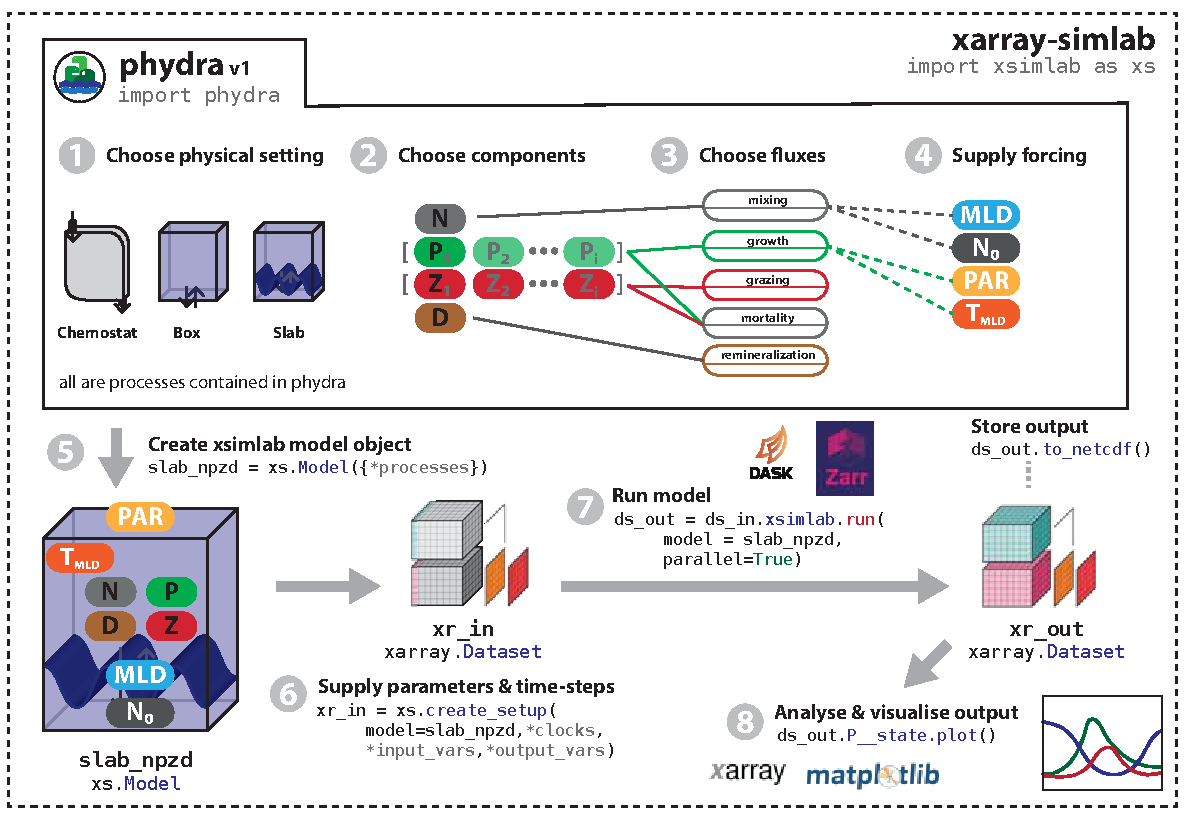
\includegraphics[width=12cm]{Figures/firstdraft_schematics/01__schematics_phydra_1.pdf}
\caption{\textit{This is slightly outdated, and will need to be updated to represent the latest version of the workflow (once the code base is fixed).} The phydra package is embedded within the xarray-simlab framework. phydra contains a library of physical settings (1), components (i.e. state variables) (2), fluxes (3) and forcing variables (4), that can be combined and reused to create an xarray-simlab model instance. Xarray-simlab provides the functionality to define the model (5) from processes in the phydra library, supply parameters and create an xarray input (6), then run the model (7) and the resulting output is dynamically stored in another xarray, with fully labelled dimensions and containing all parameters.}
\label{Figure:phydraschematics}
\end{figure*}


Phydra is a tool-box for marine ecosystem modeling, that is freely extensible by a user to be applied to many different use cases. Our goal is to make the technical implementation of writing functions and setting up a model more accessible, so that the focus can be on creating the most appropriate model structure and parameterisation for the specific scientific hypothesis that is being investigated. 

Constructing marine ecosystem models in Phydra is by design a flexible process, but the user can follow a general workflow of assembling models from the library of processes. This workflow is visualized in Figure \ref{Figure:phydraschematics} and will be further explained below.

\subsubsection{Installing and running Phydra}
The Phydra package is available via the Python pip package manager, but we encourage using Conda as a package manager that is provided with the scientific Anaconda Python distribution.
Please follow the up-to-date instructions on the Github repository for installation of Phydra and its dependencies.

% CONDA NAME DROP
Since Python and the dependencies of Phydra are constantly developed further, we will provide instructions to install a fully compatible virtual environment with the Conda package manager separate from a users standard Python installation. For interactive coding and prototyping of models using Phydra, we recommend using the Jupyter environment that is available via Conda. For more complex and larger model runs on servers Python scripts are preferable.


\subsubsection{Model creation}

To create a Phydra model object, the desired processes defining state variables, forcings and fluxes have to be provided with their corresponding label to the \texttt{phydra.Model()} function.
The model can be assembled from the Phydra library, modifications of provided base classes or custom written processes. Multiple instances of fluxes or components can easily be added to the model, as long as the provided label differentiates them.
These labels will be the specific name of the process in this model instance. At model setup, the labels are used to reference a process and provide the appropriate parameters.

When creating a model, the xarray-simlab framework automatically checks that all references between processes are fulfilled, orders the processes in their logical order of execution and returns a Phydra model object. This model object contains all processes in the model and allows the user to view all parameters required as input at model setup. The Phydra library provides several basic model objects, that can be modified by a user through a simple interface that allows removing, modifying or adding new processes.

\subsubsection{Model setup}

A Phydra model object is itself only a collection of abstract processes. In order to fully initialize a model that can be solved, the model object needs to be supplied with a complete set of parameters.

This is done using the \texttt{phydra.create\_setup()} function. The necessary arguments to this function are the model object to be setup, all required input parameters, the time range to solve the model and the specific model output to save during runtime. The Phydra setup function is a thin wrapper around the Xarray-simlab model setup function that automatically includes the solver backend and clocks setup for the chosen solving method.

Phydra provides several options to store model output, as well as storing the value of fluxes and forcings. This allows users to specify the model output that suits the complexity of the model construct. There are processes supplied that can aggregate all state variables, Forcings or Fluxes values for output storage to simplify the process of defining output. For complex functional group models the output of each component can be stored along an individually labelled dimension, while a simple NPZD model can store the output of components along a shared dimension.

The function call returns an Xarray dataset object that contains all provided parameters as well as the initialized labelled model dimensions. This dataset can be passed with the appropriate model object to be solved in the next step, but also provides an interface to exchange parameters to easily modify an already instantiated model setup.

At model setup, the xarray-simlab framework supports batch dimensions of single or multiple parameters along which the model can be solved in parallel at runtime. This provides an efficient and intuitive interface to explore the parameter space of models.

\subsubsection{Runtime}
% -> model_instance.xsimlab.run()
% relatively straightforward, this will first initialize the model data variables according to the added processes and parameters supplied, and then start model evaluation
The model setup created in the previous step already contains the necessary parameters and labelled dataset for model runtime. All that is required of the user is to call the \texttt{xsimlab.run()} attribute and provide a model object that corresponds to the model setup. This does not have to be the same model instance used to create the setup, as long as specified parameters and output are compatible.

\textit{NOTE: Currently there is only one way to solve models in Phydra: using the GEKKO dynamic sequential solver (IMODE 7).. but there are a few options to relatively easily provide an interface for other types of solvers for future versions. Not sure if I should mention the following:}

-GEKKO provides a simple interface for steady state-simulations, and model optimisation. The models constructed with Phydra are completely compatible, simply the solver process needs to be exchanged (and for model optimisation an objective function needs to be defined additionally)

- GEKKO does as of yet not provide an adaptive step size solver like odeint, but I have created a feature request and talked to the developers. This will very likely be included in future versions.




\subsubsection{Model Diagnostics and additional functionality}

- If the option is specified at setup, the model output will include not just the state variables, but the values of all fluxes. The magnitude of the fluxes can then easily be plotted...

- Xarray-simlab provides visualisation functions, that can be used to get a structured overview over all processes in a model instance. These are not optimized for the current structure though, as most dependencies between subprocesses are handled in the solver backend, not via explicit xarray-simlab process dependencies.

- Gekko stores model equations including the names of parameters and it would be possible to add some functions that print the mathematical equations.. which would be quite helpful to build and debug a model. (possible feature)

- Model optimisation (i.e. parameter fitting) is well supported by the GEKKO backend. I will run some tests, and if it works very well, it might make sense to include it in this publication, since it is a major strong point for using Phydra.


\subsubsection{Modification and further development}

The object-oriented structure of Phydra allows users to extend certain base processes to provide the desired functionality. 

Similar to how a forcing process can easily be sub-classed to supply a different type of forcing to the environment, other processes can be easily modified to have a different function, as long as the interaction between state variables matches with the dimensions and overall structure of the components involved. 

% OPEN SOURCE CONTRIBUTION 
Phydra (like Xarray-simlab and GEKKO) is an open-source project. Contributions are welcome and in fact greatly appreciated. Users can contribute in many ways by reporting bugs, submitting feedback, contributing to the development of the code or the documentation. Please read the contributing guidelines on the Github repository for further details.







%% END OF SECTION 2
\clearpage



\textit{Note: I have already written a lot of text here, then moved it to the Appendix and started writing again. I was experimenting with ways to present model structure, and currently the most finished is Use Case 1. It should be relatively easy to implement the same type of presentation for the other use cases, once the common structure is set. For a concise and complete overview of the models, please see the appendix. Sorry for the half-baked text, it probably doesn't make sense to review it in detail. Once the model example code is fully done (within the next weeks) I should be able to write this down a lot more easily.}

 %% \ SECTION 3
\section{Use cases} \label{Section:UseCases}

\begin{comment}
TODO:
- add 2 Tables for each use case, with the 1st naming all arguments to phydra.Model() and the 2nd naming all parameters supplied to phydra.create_setup()
- 

Andrew Comments:
Structure: just go through it, Use Case I, Use Case II, Use Case II. 
go through it from front to back, explain what an NPZD model is.
"We recreate the NPZD model formulation by Anderson, in the model there is one .." describe equations in words. Then say See Anderson et al. or appendix X for full equations
%  quickly explain overview, explain methods for all of them shortly, with schematics, and put full system of equations & parameter tables in the Appendix!
\end{comment}

% PARAGRAPH STARTS HERE:


% in final version, present: - jupyter notebook for each example, add links in text

% idea I had is that I actually present the models phydra style, as a collection of different processes
% a) physical env (this handles forcing)
% b) components
% c) fluxes
% d) xs.Model, xs.create_setup, xsimlab.run()

To showcase the utility of Phydra, we present three model use cases of varying complexity. In this section, we present simplified descriptions of model structure and mechanisms, following the model development workflow presented in Section \ref{Section:phydrapackage}.
Per use case, we first describe the generic physical environment employed. The environment collects the model components and computes common forcing fluxes. After describing the model components and what they represent, we move on to describe the fluxes that define the interactions between components. Finally, setup \& parameters for the model runtime are presented and simulation results are shown.

For a complete structure-independent mathematical description of the presented models please see Appendix 1. Additionally model and analysis code for all use cases is publicly available as documented interactive Jupyter notebooks in the Phydra repository (\url{https://github.com/ben1post/phydra/tree/master/examples}). 

\subsection{Use case 1: a NPZD slab model}
Our first use case presents a classical NPZD model embedded in a slab-ocean physical setting. The simplified two-layer structure provides a zero-dimensional and mechanistically simple description of physical processes affecting euphotic ecosystems in the open ocean. The classical structure lends itself well as an efficient physical test-bed for more complicated ecosystem descriptions and is often used as a teaching example.

The presented model is a slightly modified version of the elegant EMPOWER model, as presented by \citet{Anderson2015c}. 
See Figure \ref{Figure:phydraschematics_1} (a) for a schematic of the model structure and please refer to Appendix 1.1 for the full system of equations.


\subsubsection{Slab-ocean setting} \label{Section:SlabOcean}

% a) physical env (this handles forcing)
In the first and third use case, we adapt a model environment that is a slab representation of ocean physics as defined by \citet{Evans1985ACycles}. The multi-dimensional ocean is reduced to two layers, where the upper layer provides a zero dimensional setting for our ecosystem model. The bottom layer is not explicitly modeled, but often is represented by external forcings of nutrient concentrations. There is constant exchange between the layers. Nutrients are usually mixing into the upper layer, where they are consumed by phytoplankton. The fraction of all ecosystem components sinking to the bottom layer are lost from the system. These exchanges of water masses within this two-layered model ocean are driven by the empirically derived mixed layer depth (MLD). Additional common forcings that are used in slab models modify phytoplankton growth, e.g. metabolic rates via temperature and light harvesting via irradiance. Such forcing can situate a slab model theoretically in any location in the global ocean. Compared to the natural habitat of marine plankton, the slab model is a radical simplification. With the appropriate forcing the resulting simulations can yield meaningful results that can be compared with bulk properties of the marine ecosystem \cite[e.g.][]{Evans1985ACycles, Fasham1990a}.

Use cases 1 employs four types of external forcings: an external nutrient supply from below the mixed layer, (\unit{N_0}), depth of the mixed layer (MLD), photosynthetically active incident radiation (PAR) \unit{I^\emptyset} and average temperature above the mixed layer depth (\unit{T_{ML}}).

The specific forcings used here are derived from a compiled global dataset of WOA 2018 nutrient and temperature climatologies, a MLD climatology and MODIS-aqua satellite data for irradiance and chlorophyll biomass verification data. The forcing data is spatially averaged across a region of the world as specified by user input at model setup. The resulting monthly climatologies are interpolated to daily values. See Figure \ref{Figure:phydraforcing} for the two locations and specific forcings used for the presented simulations. Within the phydra structure, the slab environment supplies these forcings to fluxes that are dependent on any of these forcings. 

% PE forcing 1: mixing
We follow \citet{Evans1985ACycles} in the formulation of mixing. The change in depth of the mixed layer over time, described mathematically by the derivative of MLD, provides an estimate of mixing intensity. When MLD is shallowing (derivative is negative), the loss of component concentration is balanced with the increasing concentration due to a decreasing model volume. A deepening MLD dilutes all components (unless otherwise specified) and drives the mixing of nutrients into the upper layer.

% SEE TABLE X1 for a presentation of properties of the environment
The mixing flux in a slab environment is most often a negative term acting on components as they grow within the upper layer and sink to the unresolved deep layer. The standard mixing flux is therefore defined negatively, but the modular structure allows the creation of different mixing fluxes, with parameters that modify the effects of the generalised forcing fluxes defined in the environment, e.g. to add an additional sinking flux. The mixing flux for the nutrient component is defined separately, because it is a function of nutrient upwelling from the deeper layer via the \unit{N^\emptyset} forcing as a function of mixing and the gradient in concentration to the upper layer.

In slab models, the concentration of nutrient in the bottom layer \unit{N^\emptyset} is often assumed to be fixed. In the ocean there is usually a gradient of concentration over depth and this can be represented via functions over depth \citep{Frost1987GrazingSpp., Fasham1995VariationsAnalysis}. In this study we use an empirical climatology as the forcing \unit{N^\emptyset}, that is the result of combining WOA 2018 data with MLD climatology. From this analysis we use the WOA 2018 nitrate climatology as \unit{N^\emptyset} forcing.

% PE forcing 2: light
Another common forcing process defined in this environment, is the integrated amount of light available in the upper mixed layer. The amount of light is calculated based on the supplied PAR forcing, the current value of MLD and a function of light attenuation with ocean depth. In our model, incident irradiance is supplied by MODIS-aqua satellite climatologies. Integrated light availability in the upper mixed layer is calculated via Beer's law, dependent on MLD and the sum of extinction coefficients of water and phytoplankton biomass. 

This data provides the contrasting seasonal dynamics for the temperate and tropical location (see Figure \ref{Figure:phydraforcing}).

\subsubsection{State variables}
% b) components
Embedded with the slab environment the NPZD model contains the name-defining four ecosystem components: Nutrient (N), phytoplankton (P), zooplankton (Z) and detritus (D). 
Each model component is resolved as a single state variable. The biomass of all state variables is measured in the common model currency \unit{\mu M} of Nitrogen.

%Nutrient component
The only considered nutrient in the model system is nitrate. Nutrient is affected by the nutrient mixing flux defined in the slab physical environment.

% Phytoplankton component
A single phytoplankton state variable represents a naturally diverse phytoplankton communities. 

% Zooplankton component
A single zooplankton state variable grazes on the phytoplankton component and the detritus component.

% Detritus component
Detritus is composed of a range of organic material including faecal pellets and aggregates of marine snow of various sizes. In our model we describe an average particle of detrital matter, of which a fraction is remineralised as another fraction is sinking out of the euphotic zone and lost from the system. 



\subsubsection{Fluxes} \label{Section:SlabNPZD_Fluxes}
% c) fluxes

% PHYTOPLANKTON

% Growth flux and it's modifiers:
In the model, growth of phytoplankton is modified by three factors: Temperature, nutrient uptake and light harvesting. Multiplied by the maximum intrinsic growth rate $\mu^P$ and the current phytoplankton biomass, the growth flux is computed. 
% Temperature modifier
Temperature dependence of phytoplankton growth is calculated as the Eppley constant \citep{Eppley1972TemperatureSea}, with an exponential equivalent to a $Q_{10}$ of 1.895.
% Light limitation
In slab model simulations with a seasonally deep mixed layer, the most limiting factor during these events is often the light-dependence of phytoplankton growth. The light-limiting term is calculated via Steele's formulation \citep{Steele1962EnvironmentalSea}. Phytoplankton light limitation is further defined by an $I^{opt}$ parameter, that describes what amount of available light saturates photosynthesis, which equals phytoplankton growth in this simplified model.
% Nutrient limitation
When sufficient light is available, phytoplankton will consume nutrients. All nutrients consumed are directly incorporated into biomass. This uptake/growth rate is defined by a Monod (or Michaelis-Menten) function, showing a saturating behaviour at high nutrient availability. The maximum rate is defined by the half-saturation constant $k^N$. 
% Mortality fluxes
% here phytoplankton mortalities
Phytoplankton mortality is usually implemented as a linear rate, but we follow the EMPOWER model in resolving an additional non-linear term. A linear term describes the effects of natural mortality and metabolic loss. The added quadratic mortality represents density-dependent loss processes, such as virus induced mortalities \citep{Anderson2015c}.  
% note: EMPOWER goes into much greater detail, and cites more publications to support this.
All phytoplankton non-grazing losses contribute to detritus.




% ZOOPLANKTON
% Zooplankton grazing flux
In this simple model, zooplankton growth is not affected by environmental factors such as light or temperature.
Zooplankton grazing is the main top-down control of the phytoplankton population in our model. We follow the EMPOWER model in the choice of implementing a multiple-prey grazing formulation acting on both phytoplankton and detritus. In contrast to the grazing formulations employed by e.g. \cite{Fasham1990a}, \citeauthor{Anderson2015c} used a passive switching response, also described as a sigmoidal or Holling type 3 grazing function. The benefit of this type of grazing function over active-switching formulations is that grazing is generally proportional to food availability and the density dependence of prey preference is directly related to single prey responses \citep{Gentleman2003a}.

The zooplankton growth term is a product of total grazed phytoplankton, absorption efficiency $\beta$ and net production efficiency $\epsilon$. Using these two parameters, grazed biomass is split three ways into the fraction actually assimilated to zooplankton biomass, a fraction that is egested to detritus (e.g. faecal pellets) and another that is directly excreted as nutrient. 

% Zooplankton mortality fluxes
Similar to phytoplankton, zooplankton mortality is split into a linear term and a quadratic term. The linear term describes the natural mortality of zooplankton, that is added to the pool of detritus. The quadratic term represents the influence of higher trophic levels that are not further resolved in our zero-dimensional model. This predation-related mortality of zooplankton is assumed to be exported and lost from the system.
This term is also know as the "closure" term, since it stabilises ecosystem dynamics due to the quadratic exponent acting on the highest trophic level.

% DETRITUS
The processes adding to the pool of detritus are phytoplankton mortality, egested grazing and linear zooplankton mortality. The fraction of detritus that is remineralised each day is given by the parameter $m
^D$. In addition to being affected by mixing in the same way as phytoplankton, detritus experiences additional sinking at a rate of $v^D$ (\unit{m \ d^{-1}}).

A complete presentation of equations is given in Appendix 1.

\clearpage

\subsubsection{Model setup \& runtime}
% d) xs.Model, xs.create_setup, xsimlab.run()
The two distinct steps of model creation and model setup are presented in two tables. 


% I can resort to a more applied presentation here, actually show code?
% hm.. should this be separate from all the fluxes here? Yes, because it is together with parameters! ?
\begin{table*}[t]
\caption{Description of processes with label supplied at model creation. \textit{NOTE: what I am trying to do here is to explains the models using the specific Phydra interface, this first table is the call to phydra.Model() and the second is the call to phydra.create\_setup(). Essentially I am initializing abstract instances of the processes here, that are linked with the appropriate labels at model setup. Additional solver \& time processes are not shown here.}}
\begin{tabular}{l l}
Label & Function \\
\tophline
\textit{State variables:} \\
N & Single state variable for a component representing Nitrogen \\
P & Single state variable for a component representing Phytoplankton \\
Z & Single state variable for a component representing Zooplankton \\
D & Single state variable for a component representing Detritus \\
\\

\textit{Forcings:} \\
N0 & Forcing for nutrient concentration below ML ($N^\emptyset$) from WOA2018 climatology\\
MLD & Forcing for MLD ($H^{\mathrm{MLD}}$) from IFremer climatology\\
PAR & Forcing for PAR at surface ($I^\emptyset$) from MODIS-aqua climatology\\
Tmld & Forcing for temperature in ML ($T^{\mathrm{ML}}$) from WOA2018 climatology\\
\\

\textit{Fluxes:} \\
Mixing & Loss of component based on supplied MLD forcing \\
N\_Mixing & Mixing of nutrients based on supplied MLD and N0 forcing \\

Growth & Limited growth flux based on N, PAR and Tmld forcing \\

Grazing & Sigmoidal Holling type 3 grazing flux on multiple sources \\

P\_LinearMort & Linear mortality transferred to sink component  \\
P\_QuadMort & Quadratic mortality transferred to sink component \\
Z\_LinearMort & Linear mortality transferred to sink component \\
Z\_QuadMort & Quadratic mortality of component that is lost from system (closure) \\

D\_remin & Linear exchange flux to sink component \\
Sinking & Linear sinking flux \\
%\bottomhline
\end{tabular}
\belowtable{Abbreviations: MLD = mixed layer depth, ML = mixed layer, PAR = photosynthetically active radiation} % Table Footnotes
\label{Table:UseCase1PhysEnv}
\end{table*}
%
% there is both xs.Model and xs.create_setup.



\begin{table*}[t]
\caption{Parameters supplied at model setup \textit{NOTE: What I am trying to present here is that the model setup step requires setting parameters, as well as providing the abstract processes with the labels of processes defined in the previous step. This defines what state variables and forcings are actually used in the equations and acted upon by the fluxes. This is definitely a bit convoluted.. and I am still thinking about ways to show this more clearly... The set of parameters is also not complete. I will write the actual model example code in the next weeks. I think once that is actually written down it will be much easier to wrap my head around how to present it.}}
\begin{tabular}{l l l l l l l}
Process & Flux I/O + FX labels & Parameter & Description & Unit & Temperate & Tropical \\
\tophline

\textit{State variables:} \\
N & & $N(0)$ & initial value & \unit{µM \ N} & 1 & 1 \\
P & & $P(0)$ & initial value & \unit{µM \ N} & 1 & 1 \\
Z & & $Z(0)$ & initial value & \unit{µM \ N} & 1 & 1 \\
D & & $D(0)$ & initial value & \unit{µM \ N} & 1 & 1 \\
\\

\textit{Fluxes:} \\
Growth & N->P [I0, Tmld]& $\mu_{\emptyset}$ & maximum phytoplankton growth rate  & \unit{d^{-1}} & & \\
& & $k_N$ & half-sat. const: N uptake & \unit{µM \ N} & 0.85 & \\
P\_LinearMort & P->D & $m_P$ & linear P mortality & \unit{d^{−1}} & 0.015 & \\
P\_QuadMort & P->D & $m_{P2}$ & quadratic P mortality & \unit{(µM \ N)^{-1} d^{−1}} & 0.025 & \\
Grazing & P->Z,D,N & $I_{max}$ & Z max. ingestion rate & \unit{d^{−1}} & 1.0 & \\
&& $k_Z$ & Z half-saturation for intake & \unit{µM \ N} & 0.6 & \\
&& $\phi_P$ & grazing preference: P & & 0.67 & \\
&& $\phi_D$ & grazing preference: D & & 0.33 & \\
&& $\beta_Z$ & Z absorption efficiency & & 0.69 & \\
&& $k_{NZ}$ & Z net production efficiency & & 0.75 &  \\
Z\_LinearMort & Z->D & $m_Z$ & linear Z mortality  & \unit{d^{−1}} & 0.02 & \\
Z\_QuadMort & Z-> & $m_{Z2}$ & quadratic Z mortality & \unit{(µM \ N)^{-1} d^{−1}} & 0.34 & \\
Sinking & D-> & $v_D$ & D linear sinking rate & \unit{m \ d^{−1}} & 6.43 & \\
D\_Remin & D->N & $m_D$ & D remineralisation rate & \unit{d^{−1}} & 0.06 & \\
Mixing & P,Z,D-> [MLD]& $\kappa$ & constant mixing parameter & \unit{m \ d^{−1}} & 0.13 & \\
N\_Mixing & ->N [MLD]& $\kappa$ & constant mixing parameter & \unit{m \ d^{−1}} & 0.13 & \\ \\
%\bottomhline

\bottomhline
\end{tabular}
\belowtable{The "flux labels" are defined as source -> sink [forcing]. This actually does not relate to how they are input to phydra, it is just how I tried to simplify it visually. Each flux has parameters, like "ressource label" or "forcing label" to which the user passes a string like "N" to reference the nitrate SV in the model. Adding all of these labels as parameters above seems a bit convoluted..} % Table Footnotes
\label{Table:UseCase1Parameters}
\end{table*}
%


% Forcing setup
From the compiled global climatological forcing dataset, we chose two representative locations in the Atlantic ocean for exemplary simulations. The locations were chosen for their contrasting environmental forcings, situated in temperate (47 \unit{\degree N}, -20 \unit{\degree E}) and tropical (0 \unit{\degree N}, -20 \unit{\degree E}) climatic regions. 


\subsubsection{Results}
% keep this as dry as possible, just RESULTS no DISCUSSION
Employing the model structure, forcing and parameters presented in the previous sections, exemplary runs were conducted in two contrasting locations. 
See Figure \ref{Figure:phydraforcing} for the interpolated and raw forcing values. The temperate location shows a pronounced seasonal cycle, with a deep mixed layer depth (MLD) in winter, and high variability in light (PAR) and temperature \unit{T_{MLD}}). The tropical location shows relatively stable conditions throughout the year, and a generally lower level of nutrient concentration below the mixed layer (\unit{N^\emptyset}).

See Figure \ref{Figure:NPZDslab_results} for the temporal evolution of the four state variables for the final year of a 5 year run using repeated climatological forcing. 
The two locations show markedly different dynamics. The temperate location shows a pronounced seasonal cycle in nutrient concentration in the upper mixed layer of our model. WOA 2018 monthly climatology data of this property agrees well with the model output. Despite the relatively strong agreement between nutrient data and model output for nutrients, phytoplankton model output and a climatology of chlorophyll concentration from satellite do agree, but show a markedly different dynamic. During winter months phytoplankton biomass is reduced almost to zero in the model output. In spring, the shallowing of MLD produces a pronounced bloom, overshooting the climatological data for a short period, before it returns to levels below the data for the rest of the year. 





%%%%%%%%%%%%%%%%%%%%%%%%%%%%%%%%%%%%%%%%%%%%%%%%%%%%%%%%%%%%%%
\subsection{Use Case 2: a size-structured NPZ chemostat model}
From an attempt at describing an oceanic physical setting with a highly simplified ecosystem, we move to a simplified laboratory setting with a complex description of a size-structured ecosystem. The model structure for the second use case was adapted from \cite{Banas2011b}, with the modification that we explicitly describe the physical setting as a flow-through chemostat. See Figure \ref{Figure:phydraschematics_1} (b) for a schematic of the model structure. 


- Chemostats, a.k.a. continuous cultures, have been regularly used in exploring properties of phytoplankton! Seminal studies of Droop on nutrient uptake were performed using chemostats. \citep{Droop1968VitaminLutheri} 
- also to this day, still an interesting, very simple setting for phytoplankton models

Size is called a "master-trait" in the trait-based description of plankton ecology, allowing modellers and ecologist to describe the diverse plankton community along one continuous axis. (This is of course an oversimplification, and it takes careful consideration of the choice of allometries and often a combination of functional properties and size classes to achieve a more realistic representation of natural phytoplankton assemblages.)

See Figure \ref{Figure:phydraschematics_1} (b) for a schematic of the model structure. See Appendix 1.2 for the full system of equations.

\subsubsection{Physical environment}
\textit{Note: Here I aim to have the same kind of presentation as Use Case 1. So I describe the different model components and then show a tables with all processes initialized (Model Creation) and all parameters passed at Model Setup. If you think the way I presented Use Case 1 makes sense, I will do so. If not, I will first work out how to present Use Case 1 and then start working on this here.}

\subsubsection{Model components}

\subsubsection{Model fluxes}

\subsubsection{Model runtime}

In comparison to our first use case this model contains only three types of components (namely a nutrient, phytoplankton and zooplankton), but a much larger number of state variables (81 versus 4). The model currency is \unit{\mu M} of Nitrogen, with the only resolved nutrient being dissolved inorganic nitrogen. Additional state variables are 40 size classes of phytoplankton and 40 size classes of zooplankton. These size classes are initialised via a range of equivalent spherical diameters (ESD). For phytoplankton state variables, the ESD determines the nutrient uptake parameters, growth rates and grazing susceptibility, while for zooplankton it sets the prey range, ingestion rates and half-saturation constants of grazing. The specific size-based allometries are taken from meta-analysis of laboratory data (!refs Hansen et al 1997, Hansen et al 1994, Tang 1995, Eppley 1969). 

Thus we can initialise our model with a range of size classes. The size classes are initialised in such a way, that each phytoplankton size class is efficiently grazed by a corresponding zooplankton size class.

Mention how this means:
- there is a "type" or class of component, that uses the same functions, but with varying parameters. This technically corresponds to an array and vectorized computations in Python.
- this is what phydra excels at, flexible initialisation of component classes.

%physicalenv
A chemostat is a flow-through system that is often used in laboratories for phytoplankton growth experiments. A population of phytoplankton is inoculated in a bottle, where a constant inflow of nutrients supports their growth. As the volume is kept constant, what flows in must flow out, so a fraction of the volume containing both nutrients and phytoplankton is lost from the system continuously. The balance of nutrient supply, phytoplankton mortality and growth, as well as flow rate defines the trajectory of the system, often towards a steady state at constant flow rates. 
In this model instance, the chemostat provides the zero-dimensional setting for an NPZ ecosystem model. For mechanistic simplicity the detrital pool is not tracked and all detritus is assumed to flow out of the system before being remineralised or grazed upon.

% Nutrient dynamics
The simple physical setting describes two forcing processes, that can be described using a single variable. The chemostat provides an inflow of a nutrient solution, and at the same rate all components are flowing out of the system. The concentration of the external nutrient supply $N_0$ and the flow rate determine the amount of nutrient entering the system over time. The only additional process adding to the nutrient pool within the chemostat is excretion by zooplankton. Other fluxes, such as phytoplankton mortality and zooplankton egestion and mortality, are assumed to be removed from the system.

% Phytoplankton dynamics
Temperature and light are assumed to have no limiting effect on phytoplankton, and therefore dependent processes are not resolved in the model. Phytoplankton growth is only limited by the supply of nutrients. Similar to use case 1, nutrient uptake is instantaneously assimilated to biomass. The growth function for the phytoplankton components is made up of a size-dependent maximum growth rate and a Monod (or Michaelis-Menten) nutrient limiting-term with a size-dependent half-saturation constant multiplied by phytoplankton biomass. 
Phytoplankton losses are the constant outflux, grazing by zooplankton and a general mortality rate, that is a fraction by the size-dependent maximum growth rate $\mu^i_0$. (!ref Moloney and Field, 1991)

% Zooplankton dynamics
Zooplankton grows via assimilating ingested phytoplankton, defined as the product of growth efficiency $\epsilon$ and total ingested phytoplankton. Ingestion of each zooplankton type is a size-dependent process defined by the size of the phytoplankton prey, a half saturation constant $K_s$, the zooplankton type's specific size preference and a size-dependent maximum ingestion rate. [perhaps show a figure visualising the size-dependent allometries?]
The size preference of zooplankton types is assumed to vary with prey size in a log-Gaussian distribution around an optimal prey size for each grazer.
Width of the Gaussian distribution is controlled by the shared prey size tolerance parameter with logarithmic units.
Loss processes of zooplankton are the linear outflux and a quadratic mortality.The quadratic mortality term acts as a closure term, implicitly assuming that the rate of mortality is proportional to total zooplankton biomass (!ref Edwards and Yool, 2000). 
A fraction of grazed phytoplankton biomass, not allocated to assimilation via $\epsilon$ and egestion via $f_{eg}$, is remineralised immediately back into the nutrient state variable.

% allometric parameterisation
The allometric parameterisation follows \cite{Banas2011b}. Values of $\mu_i^\emptyset$, $I_j^\emptyset$, etc. are determined from power-law functions based on the plankton types ESD taken from review studies [add same table as BANAS 2011?].
- note caveats of allometries
- note the experimental goals of this study


\subsubsection{Results}
% JUST RESULTS NO DISCUSSION, moved to SECTION 4
% here explain the ASTroCAT model results
% note that current plot shows ASTroCAT model copy, not the chemostat modification that I have thought up (needs to be implemented and updated)

We present here the results of a 10 year model run using constant forcing in the described chemostat physical setting with one nutrient and 40 size classes of phytoplankton and zooplankton resolved. This corresponds to the base model case presented by \cite{Banas2011b} The major modification is that we moved the model system into a more explicitly theoretical chemostat setting with a constant outflow of model components. 


\subsection{Use Case 3: a size-structured NPZD slab model}
In the third use case we want to showcase flexible workflow of Phydra model development, by placing the highly resolved trophic web of use case 2 within the more realistic physical setting of use case 1. The resulting model structure is a size-structured NPZD slab model. See Figure \ref{Figure:phydraschematics_3} for a schematic of the model structure. 

- this is already quite a complex model, but there are examples of much more complex models run in global 3D settings in the literature \citep{Ward2012}
- we will compare the model output to size-fractionated phytoplankton biomass (3 size fractions: pico, nano, micro) we group phytoplankton state variables into the three size fractions (See section FORCING for more details)
- for model to data comparison, we need to adjust parameters, do parameter fitting (ideally I'll also do a sensitivity analysis with this model! should be simple using batch dims)

\subsubsection{Physical environment}

\textit{Note: As previously I want to first find a structure for Use Case 1 before working out how to present it here. This entire section is mostly copied together from the other two, and is quite rough! Still needs some work. }

\subsubsection{Model components}

\subsubsection{Model fluxes}

\subsubsection{Model runtime}

For schematic of model structure, see Figure \ref{Figure:phydraschematics_3}. Please check appendix for the system of equations. 
Since use case 3 presents no new components or processes from the previous two use case, we will not discuss mechanisms in detail, but highlight from which use case they were adapted where a more detailed description can be found. 

The model contains four ecosystem components: Nutrient, phytoplankton, zooplankton and detritus. The nutrient and detritus component are represented by a single state variable each. Planktonic components of the ecosystem are size-spectrally resolved as in use case 2.
The ecosystem is embedded in a slab physical setting as presented in use case 1. The only resolved nutrient in this system is nitrate. The concentration of all state variables is measured in the common model currency \unit{µM} of Nitrogen. Four external forcings affect the model dynamics: nitrate below the mixed layer ($N_0$), depth of the mixed layer (MLD), photosynthetically active incident radiation (PAR), average temperature above the mixed layer depth (\unit{T_{MLD}}). 

The forcings are the same interpolated monthly climatologies used for use case 1, as described in Section \ref{Section:ForcingSection}. See Figure \ref{Figure:phydraforcing} for the two locations and specific forcings applied here.

% Phytoplankton dynamics
Growth of phytoplankton is modified by three factors: Temperature, nutrient uptake and light harvesting. Multiplied by the maximum intrinsic growth rate $\mu_P$ and the current phytoplankton biomass, the growth flux is computed. Temperature dependence of phytoplankton growth is calculated as the Eppley constant \citep{Eppley1972TemperatureSea}, with an exponential equivalent to a $Q_{10}$ of 1.895.
The light-limiting term is calculated via Steele's formulation \citep{Steele1962EnvironmentalSea}. Incident irradiance is supplied by the PAR climatological forcing. Integrated light availability in the upper layer is calculated via Beer's law, dependent on MLD and the sum of extinction coefficients of water and phytoplankton biomass. Phytoplankton light limitation is further defined by an $I_{opt}$ parameter, that describes what amount of available light saturates photosynthesis.
The uptake rate of nutrients is defined by a Monod (or Michaelis-Menten) function. The maximum rate is defined by the size-dependent half-saturation constant $k^i_N$. 
% here phytoplankton mortalities
Phytoplankton mortality is implemented as a linear rate, scaled by the size-dependent maximum growth rate. 
All phytoplankton non-grazing losses contribute to detritus.

% Zooplankton dynamics
We assume that zooplankton can actively maintain themselves in the upper mixed layer and only compute diluting effects of MLD deepening, but no other mixing terms.
Zooplankton grazing is implemented with the same function (which?) described in use case 2 (see Section !3.2!) 

Zooplankton grows via assimilating ingested phytoplankton, defined as the product of growth efficiency $\epsilon$ and total ingested phytoplankton. Ingestion of each zooplankton type is a size-dependent process defined by the size of the phytoplankton prey, a half saturation constant $K_s$, the zooplankton type's specific size preference and a size-dependent maximum ingestion rate. [perhaps show a figure visualising the size-dependent allometries?]
The size preference of zooplankton types is assumed to vary with prey size in a log-Gaussian distribution around an optimal prey size for each grazer.
Width of the Gaussian distribution is controlled by the shared prey size tolerance parameter with logarithmic units.
Loss processes of zooplankton are the linear outflux and a quadratic mortality.The quadratic mortality term acts as a closure term, implicitly assuming that the rate of mortality is proportional to total zooplankton biomass (!ref Edwards and Yool, 2000). 
Only a fraction of the biomass grazed by zooplankton is assimilated to zooplankton biomass. Growth efficiency is a product of the absorption efficiency $\beta$ and net production efficiency $k_{NZ}$. Using these two parameters, grazed biomass is split three ways into the fraction actually assimilated to zooplankton, a fraction that is egested to detritus (e.g. faecal pellets) and another that is directly excreted as nutrient. 

Zooplankton mortality is split into a linear term and a quadratic term. The linear term describes the natural mortality of zooplankton, that is added to the pool of detritus. The quadratic term is assumed to be exported and lost from the system.

% Detritus dynamics
The processes adding to the pool of detritus are phytoplankton mortality, egested grazing and linear zooplankton mortality. The fraction of detritus that is remineralised each day is given by the parameter $m_D$. In addition to being affected by mixing in the same way as phytoplankton, detritus experiences additional sinking at a rate of $v_D$ (\unit{m \ d^{-1}}).

A complete presentation of equations is given in Appendix 1.

\subsubsection{Results}
% JUST RESULTS NO DISCUSSION

Using this new complex model structure, and the same forcing used for use case 1, exemplary simulations were performed in two contrasting locations. 
See Figure \ref{Figure:SizeStructuredSlab_results} for the average annual dynamics of the aggregated size-classes of 


- explain here how the runs are set up

- explain how the size class comparison works! how do i aggregate the model size classes in the plot

- these results will most likely change a lot, once the model \& package are re-coded!


\clearpage
%% Tables

\begin{table*}[t]
\caption{Allometric parameterisations and empirical parameter values employed in use case 2, adapted from \citet{Banas2011b}.}
\begin{tabular}{l l l l l}
Empirical fit & Applicability & Source \\
\tophline
$\mu_i^{\emptyset} = (2.6 \ d^{-1}) \left( \frac{size_i^{P}}{1\mu m} \right)^{-0.45}$ & Phytoplankton 1-100 ESD \unit{\mu m} & Tang(1995) \\
$k_i^N = (0.1 \ \unit{µM \ N})\left( \frac{size_i^{P}}{1\mu m} \right)$ & Phytoplankton 1-100 ESD \unit{\mu m} & Eppley et al. (1969) \\

$\mu_j^Z = (26 \ d^{-1})\left( \frac{size^i_{P}}{1\mu m} \right)^{-0.4}$ & Flagellates, dinoflagellates, ciliates, copepods & Hansen et al. (1997) \\

$k_j^Z = 3 \ \unit{µM \ N} $ & Flagellates, dinoflagellates, ciliates, copepods & Hansen et al. (1997) \\

$size_j^{opt} = (0.65 \ \unit{\mu m})\left( \frac{size^i_{P}}{1\mu m} \right)^{0.56}$ & Flagellates, dinoflagellates, ciliates, copepods & Hansen et al. (1994) \\
$\Delta size^{P} = 0.25 $ & Ciliates, nauplii, copepodites & Hansen et al. (1994)  \\
\middlehline

\bottomhline
\end{tabular}
\belowtable{TODO: the sources need to be added properly! for now just text..} % Table Footnotes
\label{appendix:table:usecase2parameters}
\end{table*}
%


\clearpage
% Figures

%%f
\begin{figure*}[t]
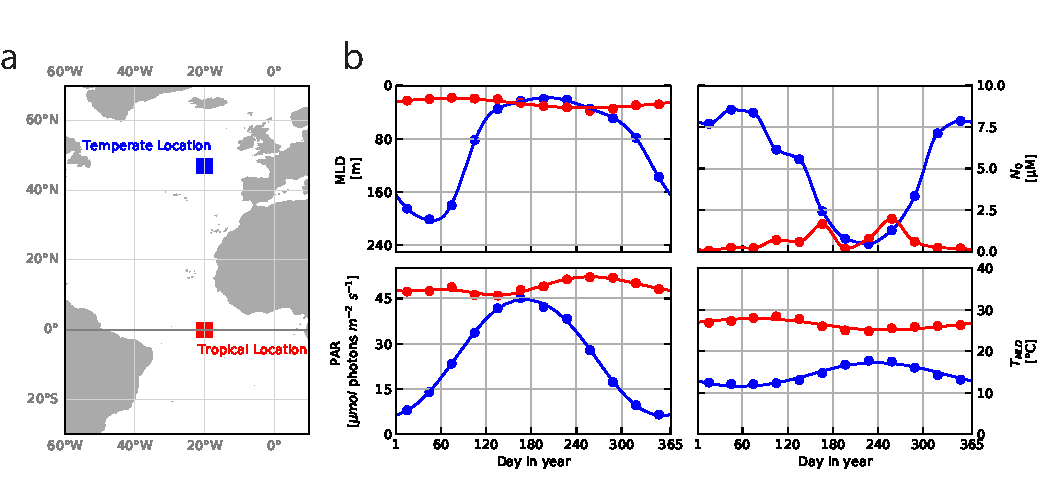
\includegraphics[width=15cm]{Figures/firstdraft_plots/01_forcing_labeled.pdf}
\caption{(a) Map shows locations of the two comparative model runs. Each square is of side length 4° centred on 47°N ,-20°E and 0°N,-20°E respectively. Environmental forcings are averaged across area. (b) Forcing is shown: Mixed Layer Depth (MLD), Nitrate below the Mixed Layer ($N_0$), Photosynthetically Active Radiation (PAR) and temperature averaged across the Mixed Layer ($T_{MLD}$)}
\label{Figure:phydraforcing}
\end{figure*}

%%f
\begin{figure*}[t]
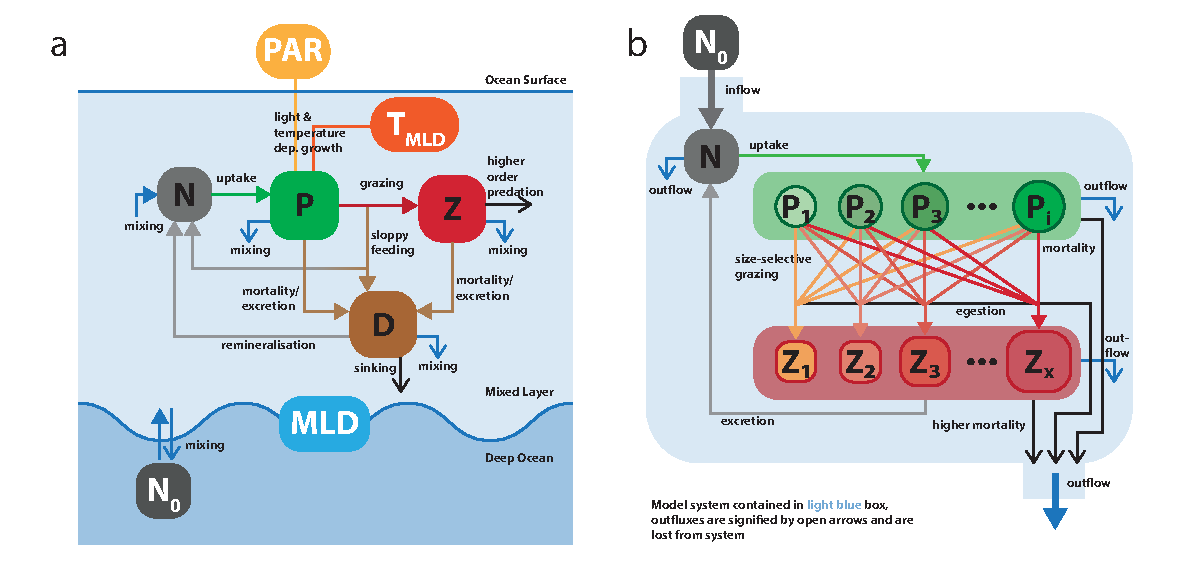
\includegraphics[width=15cm]{Figures/firstdraft_schematics/02__schematics_NPZDandChemostat.pdf}
\caption{(a) Model schematic of NPZD slab model for example 1. Model structure and parameterisation is adapted
from \citet{Anderson2015c} (b) Model schematic of size-structured $NP_{40}Z_{40}$ trophic model for use case 2. Model structure and parameterisation is adapted from \citet{Banas2011b}. [NOTE: these need to be updated, in particular with how egestion and excretion are visualised. Either both originate from grazing flux, or both are originating from "Z".. not this mixture]}
\label{Figure:phydraschematics_1}
\end{figure*}


%%f
\begin{figure}[t]
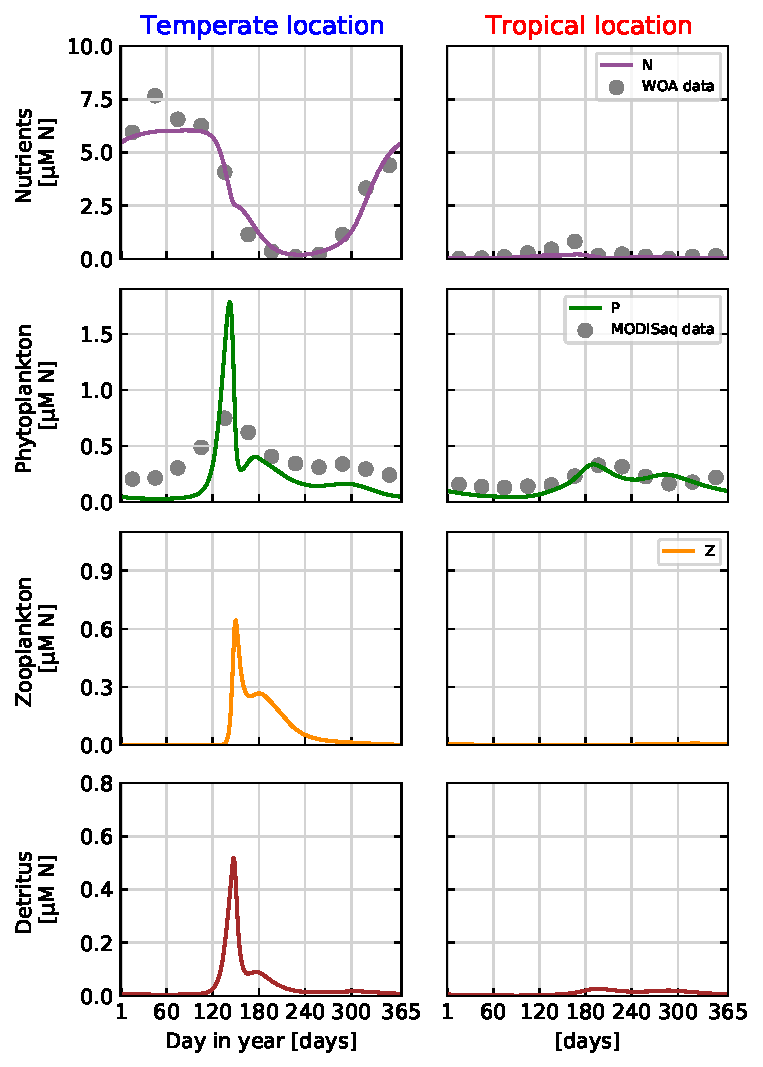
\includegraphics[width=6cm]{Figures/firstdraft_plots/02_NPZDslab.pdf}
\caption{Dynamics of NPZD slab model (i.e. use case 1) in the two exemplary locations. Output is the last year of a 5 year simulation with repeated climatological forcing. Forcing used is shown in Figure \ref{Figure:phydraforcing}. Grey dots are verification data from WOA 2018 and satellite climatology (see Section \ref{Section:ForcingSection} for details).}
\label{Figure:NPZDslab_results}
\end{figure}

%%f
\begin{figure}[t]
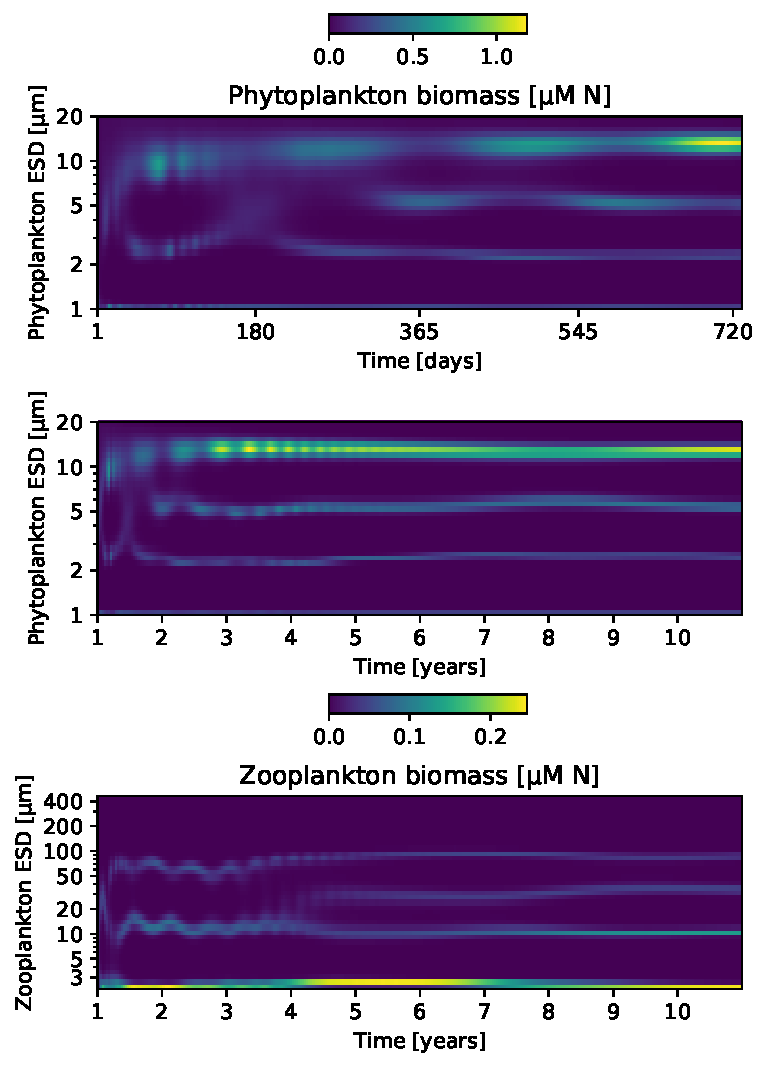
\includegraphics[width=6cm]{Figures/firstdraft_plots/03_chemostat.pdf}
\caption{Phytoplankton and zooplankton biomass per size class under steady chemostat flow-through forcing. Panel (a) shows a detailed view of the first 2 years of simulation. Panel (b) shows 10 years of model time evolution of the same run as the model output approaches a steady state. Panel (c) shows zooplankton biomass time evolution for the same model run. Plot is a recreation (same model setup \& parameters) of a plot in \citet{Banas2011b}}
\label{Figure:chemostat_plot}
\end{figure}

%%f
\begin{figure*}[t]
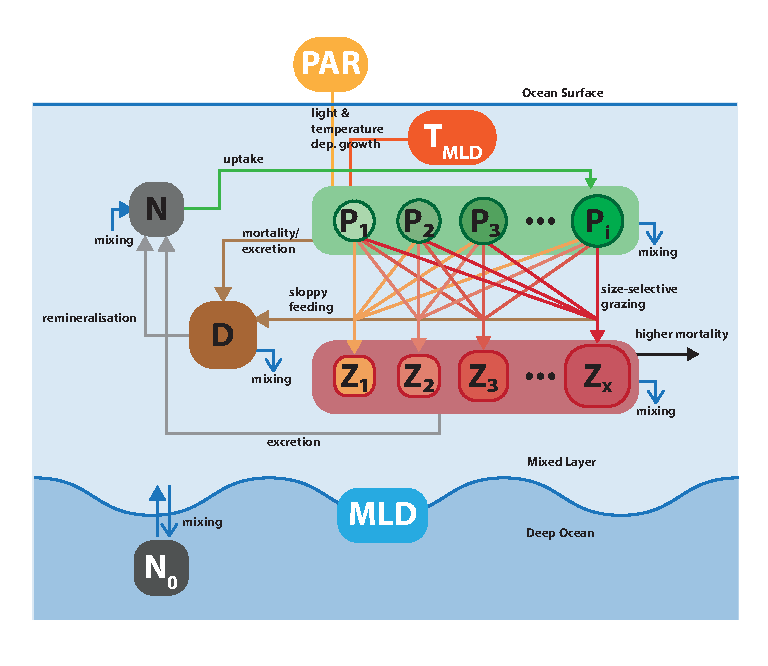
\includegraphics[width=10cm]{Figures/firstdraft_schematics/03__schematics_SizeStructSlab.pdf}
\caption{Model schematic of size-structured \unit{NP_{20}Z_{20}} slab model for use case 3. The model is a combination of the size-structured food web of use case 2 and the detritus component and slab physical setting of use case 1. The model ecosystem is contained in the light-blue area, all open errors represent loss processes that are lost from the system.}
\label{Figure:phydraschematics_3}
\end{figure*}



%%f
\begin{figure*}[t]
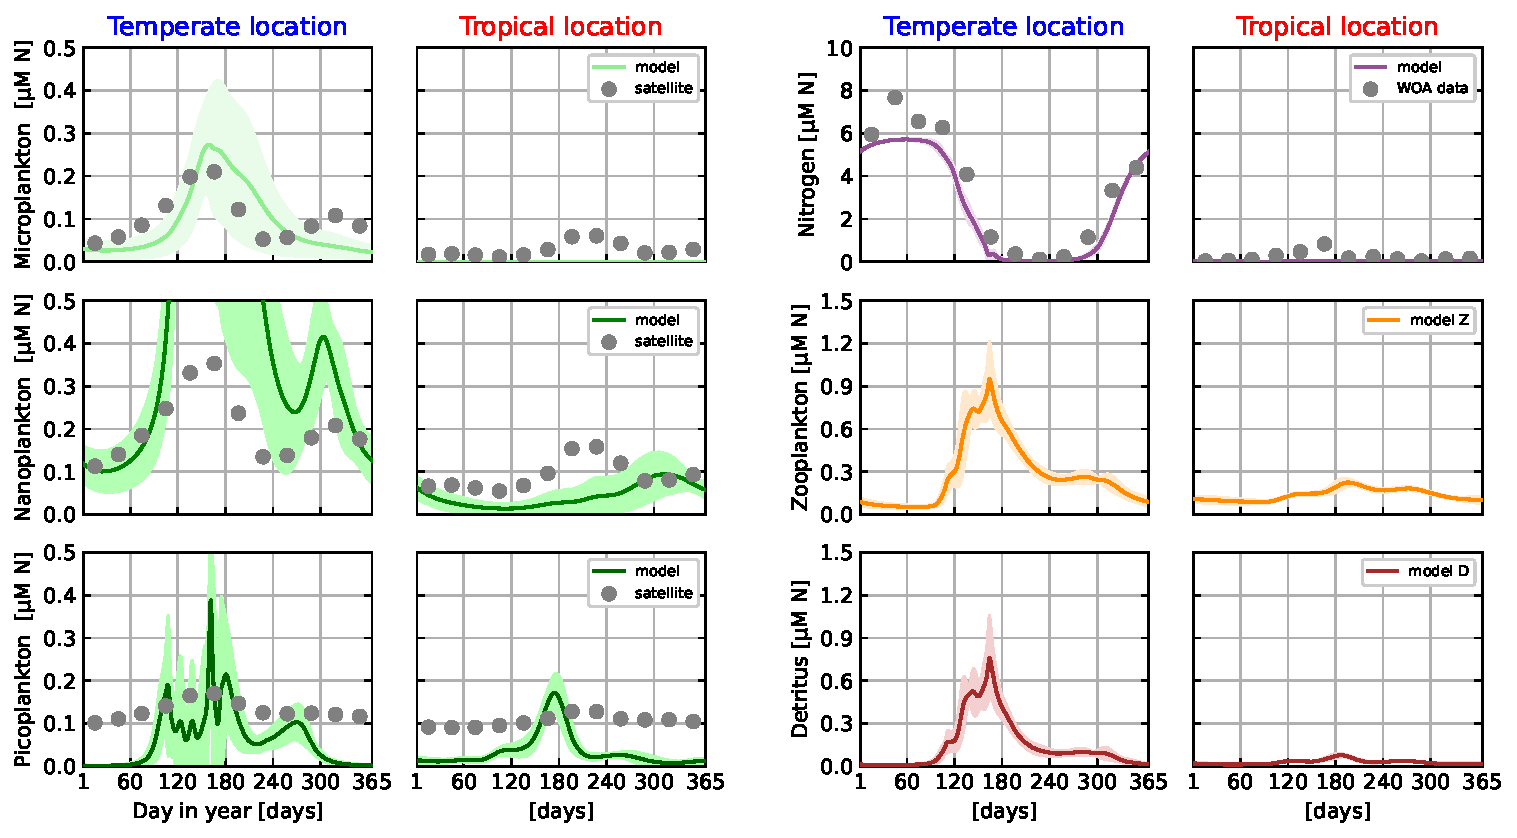
\includegraphics[width=12cm]{Figures/firstdraft_plots/04_sizestruct_slab.pdf}
\caption{Dynamics of size-structured \unit{NP_{20}Z_{20}D} slab model (i.e. use case 3) in the two exemplary locations. Solid line represents the mean dynamics of the last 10 years of a 20 year run with repeated climatological forcing, shaded areas show the standard deviation. Forcing used is shown in Figure \ref{Figure:phydraforcing}. Grey dots are verification data from WOA 2018 and satellite climatology (see Section \ref{Section:ForcingSection} for details). Size ranges are picoplankton 0.5 - 2 \unit{\mu m}, nanoplankton 2 - 20 \unit{\mu m}, microplankton 20 - 50 \unit{\mu m}. Zooplankton dynamics shown are the sum of all size classes.}
\label{Figure:SizeStructuredSlab_results}
\end{figure*}
% Tables







%%% END OF SECTION 3
\clearpage


 %% \ SECTION 4
\section{Discussion}

\textbf{ONLY ROUGH POINTS; NOT FORMULATED YET}


\begin{comment}
This is where I can actually discuss the model results, this was my idea how to keep it separate from Section 3, for a clearer reading experience.

\end{comment}

% Discussion stars here
To showcase the utility of phydra for modelling marine ecosystems, we showed three model applications of varying complexity.

Use case 1 is a canonical NPZD ecosystem model embedded in a 'slab' physical setting. The specific implementation was adapted from the elegant EMPOWER model \citep{Anderson2015c}, with simplifications to the treatment of light.

Use case 2 presents a more complex size-structured food web embedded in a simple flow-through (chemostat) setting. It is a NPZ model that resolves many size-classes of phytoplankton and zooplankton and their trophic interaction. The model structure was inspired and adapted from \citet{Banas2011b}, with modifications to the flow-through forcing. 

Use case 3 embeds the complex food web of the second use case within the 'slab' physical setting of the first. Components and processes of each previous model instance are easily combined within the phydra package, based on a common object-oriented structure. In contrast to use case 1 this model shows prolonged oscillatory inter-annual fluctuations under periodical forcing reminiscent of natural plankton populations.


\subsection{Satellite chlorophyll and nutrient climatologies as verification data}
Model verification is a very difficult process
- it usually takes specific tailoring of the model to the data, or vice versa \citep{Schartau2017}
- a good fit, does not mean a correct model \citep{RykielJr1996}

BUT, still is a basic test of model function, and for demonstration purposes.
We chose to use the Nutrient data from the WOA climatologies for nutrient concentration in the upper layer.

Additionally, we use chlorophyll climatologies from MODIS-aqua (cite!) and 

carbon-based phytoplankton size classes calculated from ocean color estimates of the particle size distribution \cite{Kostadinov2016Carbon-basedDistribution}.

The provided dataset provides an easy way to compare model output to empirical data. 

The data are highly aggregated climatologies, of poor temporal resolution (monthly). We follow this path to provide a universally useful, simple tool for marine ecosystem model development. For more specific model implementation and hypothesis testing it would be highly recommended to use local data.



\subsection{Use case 1}

This approach is perhaps mechanistically less realistic than using a photosynthesis-irradiance curve, but we chose the simpler approach without parameters dependent on chlorophyll content. For a more elaborate treatment of light in phytoplankton growth and an illuminating historical description of slab models see \citet{Anderson2015c}.


Satellites can only estimate chlorophyll concentration to visual depths, possibly extrapolated using algorithms. MLD in winter is much deeper, model output represents not concentration at surface, but concentration averaged across entire mixed layer.
The estimated chlorophyll from satellite data is converted to be compared to model output, via a constant chlorophyll-to-carbon ratio and the Redfield ratio of 16:1 (C:N), both of which are rough estimates and variable in nature. 
An ecological explanation of the observed results is that the single phytoplankton state variable represents a large diversity of organisms and can not simultaneously describe a slow-growing smaller species that survive in the winter months, as well as a larger fast-growing bloom-forming species. The model output seems to represent the latter, with it's pronounced spring bloom. 

Zooplankton and detritus state variables follow the phytoplankton biomass as would be expected from their mathematical formulation. Detritus accumulates during the phytoplankton bloom, but is otherwise readily sinking out of the mixed layer. Zooplankton only starts growing once phytoplankton biomass reaches a certain level, most likely dependent on the half-saturation constant for grazing. At lower levels, zooplankton mortality outpaces growth due to assimilated grazing. 
In realistic setting, there would always be some zooplankton and detritus within the mixed layer, but our simple model...

The tropical location shows almost no change in nutrient concentration over the year, which is not surprising giving the forcing we supply. 
Overall, the phytoplankton biomass matches satellite climatology very well 
Nutrients are depleted throughout most of the year.
Limited nutrient supply and the low phytoplankton biomass do not support much, if any, zooplankton growth and only small accumulation of detritus.

Keep in mind that these are exemplary model test runs, we do no attempt to explain the specific dynamics in these locations, just show that the model setup produces reasonable results using different forcing. Goal is not realism, but general applicability and simplicity. 


% In EMPOWER i noticed a problem with the shape model output presented in the paper and too large model time steps (due to for loop code structure, not odeint adaptive solving).. is that something I should mention, or simply forget?



differences from EMPOWER: 
Very simple model,
irradiance from satellite, not trigonometric equations. we treat light in much less detail, so say that for a more detailed treatment of light in a slab model, see \cite{Anderson2015c}

Our modifications to phytoplankton growth formulation, zooplankton mixing, as well as the treatment of forcing were adapted from the PhytoSFDM model \cite{Acevedo-Trejos2016}.
% can I say that Esteban? it is true

EMPOWER was inspired by \cite{Fasham1990a}, we stand in a long line of models. 

We hope that this simple NPZD slab model can be used as a teaching model in a similar vein to EMPOWER. The modular structure of phydra processes allows for accessible experimentation with parameterisation and model setup. 



\subsection{Use Case 2}

% here explain the ASTroCAT model results
% note that current plot shows ASTroCAT model copy, not the chemostat modification that I have thought up (needs to be implemented and updated)

We present here the results of a 10 year model run using constant forcing in the described chemostat physical setting with one nutrient and 40 size classes of phytoplankton and zooplankton resolved. This corresponds to the base model case presented by \cite{Banas2011b} The major modification is that we moved the model system into a more explicitly theoretical chemostat setting with a constant outflow of model components. Similarly to the results discussed by \cite{Banas2011b} we see a strong non-monotonicity of the planktonic ecosystem, even in such a simple environment under constant forcing. A stable size spectrum of plankton biomass appears to be reached after ~5 years of simulation, which show strong oscillatory behaviour. 
- this can be compared to natural systems
- Banas goes much deeper in analysis
- we show this as an example model ecosystem of higher complexity

Such model experiments show that the inclusion of well-resolved diversity in ecosystem models and inclusion of physiological diversity can fundamentally alter the simulated dynamics. This has repercussion far beyond theoretical systems ecology and places limits on the predictability of ecosystem dynamics (!ref Baird, 2010).


\subsection{Use Case 3}
In the previous two use cases we presented (1) a NPZD slab model containing 4 state variables within a simplified oceanic physical setting and (2) a NPZ chemostat model containing 81 state variables within a highly simplified laboratory setting. 
In the third use case we want to showcase the highly modular and flexible nature of phydra model components and processes, by placing the highly resolved trophic web of use case 2 within the more realistic physical setting of use case 1.

Using this new complex model structure, and the same forcing used for use case 1, exemplary simulations were performed in two contrasting locations. 
See Figure \ref{Figure:SizeStructuredSlab_results} for the average temporal evolution of the aggregated size-classes of 

The two locations show markedly different dynamics. The temperate location shows a pronounced seasonal cycle in nutrient concentration in the upper mixed layer of our model. 

- these results will most likely change a lot, once the model \& package are recoded!


\subsection{General Discussion}

The phydra package was designed specifically to create models of flexible dimensionality, as described in Section 2. For the presented use cases we focus varying dimensions of ecosystem complexity in relatively simple zero-dimensional physical settings. Models can be run in one, two or three-dimensional physical schemes, by providing the appropriate setup grid and processes defining physical interactions between grid points. Our choice of zero-dimensional implementations was motivated by the fact that such physical schemes are much easier to set up and analyse. The online documentation of the phydra repository (\url{https://github.com/ben1post/phydra}) provides simple examples of multi-dimensional marine ecosystem models, on which more complex implementations could be based upon.




%% END OF DISCUSSION
\clearpage



\conclusions  %% \conclusions[modified heading if necessary]
% ANDREWS COMMENTS
make the main points again (from intro)
old school modeling can be done better
show that I am moving in a direction that other people are! Brian Rose climlab, etc.

- This is a first step in the direction

- package architecture should be merged with other open-source python efforts (veros-bgcm, BGC-val)

- xsimlab is a powerful framework that is actively developed further, more added compabilities
- same goes for GEKKO

- lends itself well to interface with legacy fortran code, can make marine 3d modeling more accessible without loosing performance or accuracy

- want to make the first step, hoping that people will adopt and contribute

- any modeler willing to use phydra will probably have to write his own processes, and this is also the intention. Object oriented structure still highly simplifies collaboration with non-modelers or people not versed in higher-level python. Higher transparency and collaboration between modelers as well, since same code base and similar 

- clearly: should add 1D -> 3D example models in the future


%% END OF SECTION CONCLUSIONS



%% The following commands are for the statements about the availability of data sets and/or software code corresponding to the manuscript.
%% It is strongly recommended to make use of these sections in case data sets and/or software code have been part of your research the article is based on.

\codeavailability{TEXT} %% use this section when having only software code available


\dataavailability{TEXT} %% use this section when having only data sets available


\codedataavailability{TEXT} %% use this section when having data sets and software code available


\sampleavailability{TEXT} %% use this section when having geoscientific samples available


\videosupplement{TEXT} %% use this section when having video supplements available



\clearpage
\appendix

% appendix for Use Case 1

%' \copyrightstatement{TEXT}
\section{Use case model formulations}

\begin{comment}
Note: to allow for an intuitive depiction of multiple instances of each parameter and state variable, modifying subscripts in symbols are instead added as a superscript (e.g. $\gamma^{N}$ for the nutrient-limitation of phytoplankton growth) so that indices in the subscript signify the dimensionality of symbols (e.g. $\gamma^{N}_i$ for the term per individual phytoplankton state variable $i$). This finds no usage in use case 1, but in both 2 and 3.
Overall I attempted to make the presentation of symbols and equations coherent between use cases.
\end{comment}

In this appendix the model use cases are described mathematically, independent of their specific implementation in the phydra package. For parameter values used in model runs, please see the Tables \ref{Table:UseCase1Parameters,2,3} in Section \ref{Section:UseCases}.

\subsection{Use Case 1}

For the first use case we have implemented a traditional NPZD ecosystem model as presented in Figure \ref{Figure:phydraschematics_1} (a) with a nutrient $N$ (in this case nitrate), phytoplankton $P$, zooplankton $Z$ and detritus $D$ as state variables. The first use case model employs slab physics as presented in \citet{Evans1985ACycles}. The model ocean is built up of two layers. A biologically inert deep ocean is situated below a well mixed upper layer of variable depth that contains the ecosystem. The general model structure is adapted from the EMPOWER model presented by \citet{Anderson2015c} with simplifications to the treatment of light in the model and it's parameterisation. 
Modifications were aimed at simplifying the description of physical forcings and phytoplankton growth. The model is driven by empirical forcing describing the depth of the mixed layer ($H$), average temperature of the mixed layer ($T$), photosynthetically active radiation at the surface ($I$) and nutrient concentration in the deep layer ($N^\emptyset$) 

% modifications of EMPOWER:
%- light harvesting\\ 
%- light $PAR$ & nutrient $N^\emptyset$ forcing\\ 
%- temperature dependence of phytoplankton growth?.\\ 


\subsubsection{Mixing}

% Nutrient dynamics
The zero-dimensional physical slab setting describes two vertical layers of which the deeper layer supplies nutrients to the upper layer, whilst other components are mixed to the deep layer and lost from the system.
The magnitude of mixing is described by the coefficient $K$:

\begin{equation}
    K = \frac{h^{+} + \kappa}{H}
\end{equation}

Constant diffusive mixing is parameterized by $\kappa$. Variable mixing is a function of the change in MLD over time $h = \frac{d}{d t} H$. The derivative of MLD ($h$) is positive when the mixed layer deepens. The function $h^{+}$ defines the effects of entrainment and detrainment due to the changes in MLD as $h^{+} = \max(0, \ h)$. When the mixed layer shallows, $h^{+}$ does not modify $K$ (i.e. returns 0 instead of a negative value), based on the assumption that detrainment of mass and the increase in concentration due to the reduced volume of the mixed layer are balanced \citep{Evans1985ACycles}. 

\subsubsection{Nutrients}
Dissolved inorganic nitrogen in the mixed layer ($N$) is supplied via mixing, zooplankton excretion and detritus remineralisation.
Nutrients are entrained from the bottom layer. Mixing of nutrients is a positive term adding to $N$ along the gradient between $N^\emptyset$ and $N$. The general direction of transport is from a nutrient-rich bottom layer to the upper layer supporting phytoplankton growth, which is the only loss term.

\subsubsection{Phytoplankton}
Phytoplankton biomass ($P$) increases through temperature-dependent, light- \& nutrient-limited growth. The growth rate ($\mu^{P}$) is the product of a maximum growth rate ($\mu^{\emptyset}$) and the growth-dependencies on temperature ($\gamma^{T}$), light ($\gamma^{I}$) and nutrients ($\gamma^{N}$): 

\begin{equation}
    \mu^{P} = \mu^{\emptyset} \ \gamma^{T} \ \gamma^{I} \ \gamma^{N}
\end{equation}

$T$ is the average temperature of the mixed layer in \unit{\degree C}, as supplied from model forcing. Temperature dependence of the growth rate ($\gamma^{T}$) is calculated via the Eppley curve \citep{Eppley1972TemperatureSea}, with an exponential equivalent to a $Q_{10}$ of 1.895.

\begin{equation}
    \gamma^{T} = \exp{(0.063 \ T)} \label{mumax}
\end{equation}

The light-limiting term $\gamma^{I}$ represents growth-dependence on total light ($I$) available to phytoplankton the upper mixed layer. We use a simplified form of Steele's formulation to describe light-limitation of phytoplankton growth in the mixed layer, as adapted from \citet{Acevedo-Trejos2016} and originally described in \citet{Steele1962EnvironmentalSea}.

\begin{equation}
    \gamma^{I} = \frac{1}{H} \int_{0}^{H}\left[ \frac{I(z)}{I^{opt}} \cdot \exp{\left( 1 - \frac{I(z)}{I^{opt}} \right) }  \right]dz \label{steele1}
\end{equation}

Where $I^{opt}$ is the light level at which photosynthesis saturates and $I(z)$ is the irradiance at depth $z$.
The irradiance forcing $I$ is a temporally and spatially averaged monthly climatology of photosynthetically active radiation (PAR) at the surface. 

Attenuation of $I$ at depth $z$ in the mixed layer is calculated according to the Lambert-Beer equation:

\begin{equation}
    I(z) = I \ \exp{(-k^{PAR} \ z)} \label{beer}
\end{equation}

The attenuation coefficient $k^{PAR}$ is the sum of the attenuation coefficient of seawater $k^w$ and that of phytoplankton biomass $k^c$, which is multiplied by the current phytoplankton biomass $P$:

\begin{equation}
    k^{PAR} = k^w + k^c \cdot P
\end{equation}

Combining the equations and integrating across the mixed layer, the numerical solution for the integrated light-limiting term affecting phytoplankton growth is calculated. Integrated values within the mixed layer larger than the optimal irradiance will limit growth, to model effects of photo-inhibition \citep{Steele1962EnvironmentalSea}.
This simple implementation uses only one parameter to describe light limitation of phytoplankton growth, which is $I^{opt}$. This is a highly simplified treatment of light in a slab model. A more realistic representation of light-limited growth would include chlorophyll-to-biomass ratios and related parameters and functions. See \citet{Anderson2015c} for an insightful discussion of light-limitation in slab models.

Nutrient limitation of phytoplankton growth $\gamma^N$ is described by the Michaelis-Menten (or Monod) equation.

\begin{equation}
    \gamma^N = \frac{N}{k^N + N}
\end{equation}

where $k^N$ is the half-saturation constant for nutrient uptake. $N$ is the ambient nutrient concentration, in this case of dissolved inorganic nitrogen (DIN). In this simple model there is no distinction between nutrient uptake and assimilation of nutrient via growth.

Non-grazing mortality of phytoplankton is described by both a linear $m^P$ and a quadratic factor $m^{P2}$ \citep{Yool2011Medusa-1.0:Domain}. The former accounts for natural mortality and excretion. Quadratic mortality describes density-dependent loss processes, which can be caused by viral infection. All non-grazing loss terms feed into the detritus pool.

\subsubsection{Zooplankton}
Grazing by zooplankton occurs on both phytoplankton and detritus. The grazing function is a Holling Type 3 grazing response as presented in \citet{Anderson2015c}:

\begin{equation}
    G^P = \mu^Z \left( \frac{ \hat{\phi}^P P}{(k^Z)^2 + \hat{\phi}^D D +\hat{\phi}^P P}  \right) Z
\end{equation}
where $\hat{\phi}^P$ = $\phi^P \ P$, $\hat{\phi}^D$ = $\phi^D \ D$.

This formulation describes the total biomass of phytoplankton that is grazed $G^P$. Parameter $\mu^Z$ is the maximum ingestion rate for a food source, in this case both phytoplankton and detritus. 
The grazing preference parameters $\phi^P$ and $\phi^D$ do not represent a discrete fraction of the amount grazed in the diet relative to the environment. Instead, this amount is represented by the ratio of $\hat{\phi}^P$ and $\hat{\phi}^D$. 
The half-saturation constant for grazing $k^Z$ is similarly an arbitrary parameter, that scales the density-dependent half-saturation constant $k^P$ for grazing on phytoplankton based on the choice of $\phi^P$, with the relationship $k^P$ = $\sqrt{\frac{(k^Z)^2 }{ \phi^P}}$.


Similarly the detritus grazing flux is defined as:

\begin{equation}
    G^D = \mu^Z \left( \frac{ \hat{\phi}^D D}{(k^Z)^2 + \hat{\phi}^D D +\hat{\phi}^P P}  \right) Z
\end{equation}

This sigmoidal response includes passive prey switching via an interference effect, where the increase in biomass of one prey slightly reduces the intake of other prey. In contrast to other grazing formulations \citep[e.g.][]{Fasham1990a}, the prey switching mechanism does not create sub-optimal feeding, where an increase in biomass of less common prey can decreases the total grazing flux \citep{Gentleman2003a}.

Zooplankton ingestion of prey does not directly convert to biomass gained however. The total biomass grazed ($G^P + G^D$) is split three ways between zooplankton growth (to $Z$), excretion of dissolved nutrients (to $N$) and egestion of faecal matter \& particles (to $D$). Zooplankton growth is a product of total biomass grazed ($G^P$) and the gross growth efficiency (GGE) of zooplankton. The two parameters defining GGE in this model are absorption efficiency ($\beta$) and net production efficiency ($\epsilon$). Adsorption efficiency $\beta$ describes the fraction of $G^P$ which is absorbed in the gut, of which the fraction $\epsilon$ is actually assimilated into biomass (to $Z$: \ $\beta \epsilon$), while the rest is excreted as DIN (to $N$: \ $\beta (1-\epsilon)$). GGE specifically is the product of $\epsilon$ and $\beta$, for which values between 0.2 and 0.3 have been observed for a wide range of zooplankton \citep{Straile1997GrossGroup}. The fraction of $G^P$ egested to $D$ (e.g. as faecal pellets) is calculated via $1-\beta$. 

Similar to phytoplankton mortality, the linear mortality factor $m^Z$ parameterizes natural mortality and excretion and feeds into the pool of detritus. The quadratic factor $m^{Z2}$ describes higher order predation on zooplankton and is removed from the system. 

\subsubsection{Detritus}
Detritus concentration in the upper layer ($D$) is supplied by all mortality of phytoplankton, linear zooplankton mortality and zooplankton egestion (e.g. faecal pellets). The loss terms are remineralisation, zooplankton grazing, mixing and an additional sinking flux. 

Detritus is remineralised at a constant rate $m^D$. Similar to $P$ and $Z$, $D$ is affected by mixing through changes in MLD, described by the mixing coefficient $K$. In addition to $K$, detritus experiences losses due to gravitational sinking at a rate of $v^D$. This term is added to describe the fast export of larger detritus particles below the mixed layer. 

\clearpage
\subsubsection{Model equations}
The rates of change of the state variables are described by the following set of equations. For the definition of all symbols used here see Table \ref{appendix:table:usecase1symbols}. See \citet{Anderson2015c} for a more detailed discussion of model structure and formulation.

\begin{equation}
    \frac{d N}{d t} = 
    K (N^\emptyset - N) % Nutrient mixing
    + \beta(1 - \epsilon)(G^P + G^D) % Unassimilated grazing by Z
    + m^D \ D % Remineralisation of D
    - \mu^{P} \ P % Phytoplankton gains
\end{equation}

%PHYTOPLANKTON
\begin{equation}
    \frac{d P}{d t} =
    \mu^{P} \ P  % Phytoplankton gains
    - m^P \ P % Linear mortality
    - m^{P2} \ (P)^2 % Quadratic mortality
    - G^P % Z grazing
    - K \ P % Phytoplankton mixing
\end{equation}

%ZOOPLANKTON
\begin{equation}
    \frac{d Z}{d t} =
    \beta \ \epsilon(G^P + G^D) % Assimilated grazing
    - m^Z \ Z % Linear mortality
    - m^{Z2} \ (Z)^2 % Quadratic mortality
    - K \ Z % Zooplankton mixing
\end{equation}

%DETRITUS
\begin{equation}
    \frac{d D}{d t} = 
    m^P \ P % Linear mortality
    + m^{P2} \ (P)^2 % Quadratic mortality
    + m^Z \ Z % Linear mortality
    + (1 - \beta)(G^P + G^D) % Unassimilated grazing by Z
    - G^D % Z grazing on D
    - m^D \ D % Remineralisation of D
    - K \ D % Mixing of D
    - \frac{v^D}{H} \ D % Sinking of D
\end{equation}



\clearpage
%TABLES & FIGURES



\begin{table*}[t]

\caption{ Definition of symbols employed in use case 1 appendix. (\unit{\mu M \ N} = \unit{mmol \ Nitrogen \ m^{-3}}) }

\begin{tabular}{l l l}
Symbol & Meaning & Unit\\
\tophline
\tophline
State variables:\\
\middlehline
$N$ & concentration of nutrient in the upper mixed layer & \unit{\mu M \ N} \\
$P$ & concentration of phytoplankton biomass in the upper mixed layer & \unit{\mu M \ N} \\
$Z$ & concentration of zooplankton biomass in the upper mixed layer & \unit{\mu M \ N} \\
$D$ & concentration of detritus in the upper mixed layer & \unit{\mu M \ N} \\

Forcings:\\
\middlehline
$N^\emptyset$ & nutrient concentration right below mixed layer & \unit{\mu M \ N} \\
$H$ & depth of the upper mixed layer (MLD) & \unit{m} \\
$h^+$ & positive derivative of H(t) & \unit{m \ d^{−1}}  \\
$I$ & irradiance at the surface & \unit{\mu mol \ photons \ m^{-2} \ s^{-1}} \\
$T$ & temperature of the upper mixed layer & \unit{\degree C} \\
Processes:\\
\middlehline
$K$ & material exchange between mixed and bottom layer & \unit{m \ d^{-1}} \\
$\gamma_T$ & temperature dependency of phytoplankton growth & dimensionless \\
$\gamma_I$ & light limitation of phytoplankton growth &  dimensionless\\
$\gamma_N$ & nutrient limitation of phytoplankton growth & dimensionless \\
$G_P$ & total biomass of phytoplankton grazed by zooplankton & \unit{\mu M \ N} \\
$G_D$ & total biomass of detritus grazed by zooplankton & \unit{\mu M \ N} \\
Parameters: \\
\middlehline
$\kappa$ & constant mixing parameter & \unit{m \ d^{−1}}  \\
$v^D$ & additional sinking parameter & \unit{m \ d^{−1}}  \\
$\mu^\emptyset$ & maximum phytoplankton growth rate & \unit{d^{−1}}  \\
$I^{opt}$ & constant mixing parameter & \unit{\mu mol \ photons \ m^{-2} \ s^{-1}}  \\
$k^w$ & light attenuation constant of sea water & \unit{m^{−1}}  \\
$k^c$ & light attenuation constant of phytoplankton biomass & \unit{m^{−1}}  \\
$k^N$ & half-saturation constant for nutrient uptake & \unit{\mu M \ N}  \\
$\mu^Z$ & maximum ingestion rate of zooplankton & \unit{d^{−1}}  \\
$\phi_P$ & zooplankton grazing preference for phytoplankton & dimensionless \\
$\phi_D$ & zooplankton grazing preference for zooplankton & dimensionless \\
$k_Z$ & half-saturation constant for zooplankton intake & \unit{\mu M \ N} \\
$\beta$ & absorption efficiency of zooplankton grazing &  dimensionless \\
$\epsilon$ & net production efficiency of zooplankton grazing & dimensionless \\
$m^D$ & remineralisation rate of detritus & \unit{d^{-1}} \\
$m^P$ & linear mortality of phytoplankton & \unit{d^{-1}} \\
$m^{P2}$ & quadratic mortality of phytoplankton & \unit{(\mu M \ N)^{-1} \ d^{-1}} \\
$m^Z$ & linear mortality of zooplankton & \unit{d^{-1}} \\
$m^{Z2}$ & quadratic mortality of zooplankton & \unit{(\mu M \ N)^{-1} \ d^{-1}} \\
%\middlehline
%\bottomhline
\end{tabular}
\label{appendix:table:usecase1symbols}
%\belowtable{This is a test} % Table Footnotes
\end{table*}



\clearpage
% appendix for Use Case 2

\subsection{Use Case 2}

For the second use case we have implemented a size-spectral NPZ ecosystem model as presented in Figure \ref{Figure:phydraschematics_1} (b) with a nutrient $N$ (in this case nitrate), multiple size classes of both phytoplankton $P_i$ and zooplankton $Z_j$ as state variables. 
This model use case employs a simple chemostat as physical setting. A flow-through culture, where organisms grow in a bottle with a continuous influx of a nutrient solution. At the same rate all components of the bottle flow out of the system, so that volume remains constant over time.
Model structure and parameterisation is adapted from the ASTroCAT model \citep{Banas2011b}, with slight modifications to the physical environment and parameterisation. 

The model describes a size-structured community of phytoplankton and zooplankton, with each state variable defined by their equivalent spherical diameter (ESD). In model runs presented in this paper, we follow \citet{Banas2011b} in running simulations with 40 size classes of equally log-spaced ESD of $P$ (1 to 20 \unit{\mu m}), and 40 matching classes of $Z$ (2.1 to 460  \unit{\mu m}). 
The model can be defined with any number of size classes within meaningful boundaries of the allometric parameterisation. Size classes are denoted by the subscript $i$ for phytoplankton and $j$ for zooplankton. In the implementation of a size-spectral model by \citeauthor{Banas2011b} the food-web is implicitly made up of pairs of $P_i$ and $Z_j$, to avoid creating classes at the ends of the size spectrum that are artificially released or suppressed by grazing pressure.

The main modification to the model structure in ASTroCAT is the physical setting. An additional outflow acts as a loss term on all model components to place them in a traditional experimental setting for phytoplankton ecology, a chemostat system.

\subsubsection{Flow}

Nutrient supply to the system is defined by a linear flow rate $f$ and the nutrient concentration in the supplied solution $N^\emptyset$. All components, including phytoplankton and zooplankton are lost from the system at the same rate $f$.

\subsubsection{Nutrient}
Dissolved inorganic nitrogen (DIN) in the model system ($N$) is supplied from influx of medium (with nutrient concentration $N^\emptyset$) at a constant rate $f$ and the fraction of grazed biomass that is excreted by $Z$. The concentration $N^\emptyset$ and the flow rate $f$ determine the total nutrient supply to the system. At the same rate $N$ is flowing out from the system. Zooplankton excretion is a recycled term, that also adds back into the pool of $N$. The major loss term to $N$ is phytoplankton growth.

\subsubsection{Phytoplankton}
Phytoplankton biomass $P$ increases through  nutrient-limited growth. Nutrient limitation of phytoplankton growth $\gamma_i^N$ is described by the Michaelis-Menten (or Monod) equation:

\begin{equation}
    \gamma_i^N =  \frac{N}{k_i^N + N} 
\end{equation}

where $k_i^N$ is the size-dependent half-saturation constant. $N$ is ambient nutrient concentration in the medium.

Non-grazing mortality of phytoplankton is described the factor $m^P$ that is scaled by the maximum intrinsic growth rate $\mu_i^{\emptyset}$. This accounts for natural mortality and excretion.

\subsubsection{Zooplankton}
Zooplankton size class $j$ grazing on phytoplankton size class $i$ is calculated by
\begin{equation}
    G_{ij}^P = \mu_j^Z \ \frac{ \phi_{ij} \cdot P_i }{ k_j^Z + \sum_{i}(\phi_{ij} \cdot P_i) } \ Z_j
\end{equation}
where $\mu_j^Z$ is the size-dependent maximum ingestion rate, $k_j^Z$ is the prey half-saturation level and $\phi_{ij}$ is the relative preference of $Z_j$ for prey type $P_i$.

Prey preference is assumed to vary with phytoplankton size $size_i^{P}$ in a log-Gaussian distribution around an optimal prey size for each grazer $size_j^{opt}$.

\begin{equation}
    \phi_{ij} = exp \left[ -\left( \ \frac{ log_{10}(size_i^{P}) - log_{10}(size_j^{opt}) }{ \Delta size^{P} } \right) \right]
\end{equation}
Where $\Delta size^{P}$ is the prey size tolerance parameter, with units of \unit{log_{10}(\mu m)}, that controls the width of the Gaussian distribution.

Zooplankton growth is a product of total biomass grazed ($G^P$) and the gross growth efficiency (GGE) of zooplankton. The two parameters defining GGE in this model are absorption efficiency ($\beta$) and net production efficiency ($\epsilon$). Adsorption efficiency $\beta$ describes the fraction of $G^P$ which is absorbed in the gut, of which the fraction $\epsilon$ is actually assimilated into biomass (to $Z$: \ $\beta \epsilon$), while the rest is excreted as DIN (to $N$: \ $\beta (1-\epsilon)$). GGE specifically is the product of $\beta$ and $\epsilon$, for which values between 0.2 and 0.3 have been observed for a wide range of zooplankton  \citep{Straile1997GrossGroup}. The fraction of $G^P$ egested (e.g. as faecal pellets) is calculated via $1-\beta$, which in the current model setup is assumed to be exported quickly in the flow-through setting and lost from the system. 

Zooplankton experiences quadratic mortality according to the parameter $m^{Z2}$, describing higher-order mortality and predation of zooplankton that is removed from the system \citep{Edwards2000TheModels}. This closure term is quadratic, calculated with the implicit assumption that mortality of $Z_j$ is proportional to total zooplankton biomass $\sum_{j} Z_j$.

\clearpage
\subsubsection{Model equations}
The rates of change of the state variables are described by the following set of equations. For the definition of all symbols used here see Table \ref{appendix:table:usecase2symbols}.
See \citet{Banas2011b} for a more detailed discussion of model structure and formulation. 

\begin{equation}
    \frac{d N}{d t} = 
    f \ N^\emptyset % Nutrient mixing
    +  \beta (1 - \epsilon) \sum_{j} \sum_{i} G_{ij}^P % Unassimilated grazing by Z
    - \sum_{i} ( \mu_i^{\emptyset} \ \gamma_i^N \ P_i) % Phytoplankton gains
    - f \ N
\end{equation}

%PHYTOPLANKTON
\begin{equation}
    \frac{d P_i}{d t} =
    \mu_i^{\emptyset} \  \gamma_i^N \   P_i  % Phytoplankton gains
    - m^P  \ \mu_i^{\emptyset} \ P_i % Linear mortality
    - \sum_{j} G_{ij}^P % Z grazing
    - f \ P_i
\end{equation}

%ZOOPLANKTON
\begin{equation}
    \frac{d Z_j}{d t} =
    \beta \ \epsilon \ \sum_{i} G_{ij}^P % Assimilated grazing
    - m^{Z2} \ Z_j \ \sum_{j} Z_j  % Quadratic mortality
    - f \ Z_j
\end{equation}




\clearpage
%TABLES & FIGURES


\begin{table*}[t]

\caption{ Definition of symbols employed in use case 2 appendix. (\unit{\mu M \ N} = \unit{mmol \ Nitrogen \ m^{-3}}) }

\begin{tabular}{l l l}
Symbol & Meaning & Unit\\
\tophline
\tophline
State variables:\\
\middlehline
$N$ & concentration of nutrient in model system & \unit{\mu M \ N} \\
$P_i$ & concentration of phytoplankton size class $i$ biomass  & \unit{\mu M \ N} \\
$Z_j$ & concentration of zooplankton size class $j$ biomass  & \unit{\mu M \ N} \\


Forcings:\\
\middlehline
$f$ & flow-through rate of chemostat environment (influx \& outflux) & \unit{d^{-1}} \\
$N_0$ & nutrient concentration of source medium for chemostat & \unit{\mu M \ N} \\



Processes:\\
\middlehline
$\gamma_i^N$ & nutrient-dependence of the growth of phytoplankton size class $i$ & dimensionless\\
$G_{ij}^P$ & total biomass of phytoplankton size class $j$ grazed by zooplankton size class $i$ & \unit{\mu M \ N} \\
$\phi_{ij}$ & Preference of grazer $Z_j$ for prey $P_i$ & dimensionless \\


Parameters: \\
\middlehline
$\mu_i^{\emptyset}$ & size-dependent max. growth rate of phytoplankton & \unit{d^{-1}} \\
$k_i^N$ & Phytoplankton size class $i$ half-saturation constant for nutrient uptake & \unit{\mu M \ N} \\
$m^P$ & fraction of size-dependent $\mu_i^{\emptyset}$ that is phytoplankton mortality & dimensionless \\

$\mu_j^Z$ & maximum ingestion rate for zooplankton size class $j$ &  \unit{d^{-1}} \\

$k_j^Z$ & Prey half-saturation level for zooplankton size class $j$ & \unit{\mu M \ N} \\
$size_i^{P}$ & Individual size of phytoplankton (prey) size class $i$ & \unit{\mu m} \\
$size_j^{opt}$ & Optimal prey size for zooplankton size class $j$ & \unit{\mu m} \\
$\Delta size^{P}$ & Prey size tolerance for grazers & \unit{log_{10}(\mu m)} \\

$\beta$ & absorption efficiency of zooplankton, fraction of $G_{ij}^P$ &  dimensionless \\
$\epsilon$ & net production efficiency of zooplankton, fraction of $\beta$ & dimensionless \\

$m^{Z2}$ & quadratic mortality of zooplankton, dependent on total $Z$ biomass & \unit{(\mu M \ N)^{-1} \ d^{-1}} \\

%\middlehline
%\bottomhline
\end{tabular}
\label{appendix:table:usecase2symbols}
%\belowtable{This is a test} % Table Footnotes
\end{table*}

%%%%%%%%%%%%%%%%



\clearpage
% appendix for Use Case 3

\subsection{Use Case 3}

For the third case the model structure is a combination of the previous two use cases. The result is a size-structured NPZD slab model, as presented in Figure \ref{Figure:phydraschematics_3} with a nutrient $N$, multiple size classes of both phytoplankton $P_i$ and zooplankton $Z_j$ and detritus $D$ as state variables.
This ecosystem is embedded in a slab physical setting, as per \citet{Evans1985ACycles}. The model ocean is built up of two layers. A biologically inert deep ocean is situated below a well mixed upper layer of variable depth that contains the ecosystem. 

The general model structure is adapted from the EMPOWER model presented by \citet{Anderson2015c}. Modifications to the formulation, were aimed at simplifying the description of physical forcings and phytoplankton growth (see Section A 1.1 for further detail). We replace the singular $P$ and $Z$ state variables, with the diverse $P_i$ and $Z_j$ and their size-structured trophic web as defined Appendix 1.2 and adapted from \citet{Banas2011b}. The model is driven by empirical forcing describing the depth of the mixed layer ($H$), average temperature of the mixed layer ($T$), photosynthetically active radiation at the surface ($I$) and nutrient concentration in the deep layer ($N^\emptyset$).

The model ecosystem describes a size-structured community of phytoplankton and zooplankton, with each state variable defined by their equivalent spherical diameter (ESD). In model runs presented in this paper, we follow \citet{Banas2011b} in running simulations with 40 (or 20?) size classes of equally log-spaced ESD of $P$ (1 to 20 \unit{\mu m}), and 40 (?)  matching classes of $Z$ (2.1 to 460  \unit{\mu m}). 
Size classes are denoted by the subscript $i$ for phytoplankton and $j$ for zooplankton. In the implementation of a size-spectral model by \citeauthor{Banas2011b} the food-web is implicitly made up of pairs of $P_i$ and $Z_j$, to avoid creating classes at the ends of the size spectrum that are artificially released or suppressed by grazing pressure.



\subsubsection{Mixing}
% Nutrient dynamics
The zero-dimensional physical slab setting describes two vertical layers of which the deeper layer supplies nutrients to the upper layer, whilst other components are mixed to the deep layer and lost from the system.
The magnitude of mixing is described by the coefficient $K$:

\begin{equation}
    K = \frac{h^{+} + \kappa}{H}
\end{equation}

Constant diffusive mixing is parameterized by $\kappa$. Variable mixing is a function of the change in MLD over time $h = \frac{d}{d t} H$. The derivative of MLD ($h$) is positive when the mixed layer deepens. The function $h^{+}$ defines the effects of entrainment and detrainment due to the changes in MLD as $h^{+} = \max(0, \ h)$. When the mixed layer shallows, $h^{+}$ does not modify $K$ (i.e. returns 0 instead of a negative value), based on the assumption that detrainment of mass and the increase in concentration due to the reduced volume of the mixed layer are balanced \citep{Evans1985ACycles}. 


\subsubsection{Nutrients}
Dissolved inorganic nitrogen in the mixed layer ($N$) is supplied via mixing, zooplankton excretion and detritus remineralisation.
Nutrients are entrained from the bottom layer. Mixing of nutrients is a positive term adding to $N$ along the gradient between $N^\emptyset$ and $N$. The general direction of transport is from a nutrient-rich bottom layer to the upper layer supporting phytoplankton growth, which is the only loss term.


\subsubsection{Phytoplankton}
Phytoplankton size-class biomass ($P_i$) increases through temperature-dependent, light- \& nutrient-limited growth. The growth rate ($\mu_i^{P}$) is the product of a size-dependent maximum growth rate ($\mu_i^{\emptyset}$) and growth-dependency on nutrients ($\gamma_i^{N}$), as well as the general growth dependencies  on temperature ($\gamma^{T}$), light ($\gamma^{I}$) that are shared between size classes: 

\begin{equation}
    \mu_i^{P} = \mu_i^{\emptyset} \ \gamma^{T} \ \gamma^{I} \ \gamma_i^{N}
\end{equation}

$T$ is the average temperature of the mixed layer in \unit{\degree C}, as supplied from model forcing. Temperature dependence of the growth rate ($\gamma^{T}$) is calculated via the Eppley curve \citep{Eppley1972TemperatureSea}.

\begin{equation}
    \gamma^{T} = \exp{(0.063 \ T)} \label{mumax2}
\end{equation}

The light-limiting term $\gamma^{I}$ represents growth-dependence on total light ($I$) available to phytoplankton the upper mixed layer. We use a simplified form of Steele's formulation to describe light-limitation of phytoplankton growth in the mixed layer, as adapted from \citet{Acevedo-Trejos2016} and originally described in \citet{Steele1962EnvironmentalSea}.

\begin{equation}
    \gamma^{I} = \frac{1}{H} \int_{0}^{H}\left[ \frac{I(z)}{I^{opt}} \cdot \exp{\left( 1 - \frac{I(z)}{I^{opt}} \right) }  \right]dz \label{steele}
\end{equation}

Where $I^{opt}$ is the light level at which photosynthesis saturates and $I(z)$ is the irradiance at depth $z$.
The irradiance forcing $I$ is a temporally and spatially averaged monthly climatology of photosynthetically active radiation (PAR) at the surface. 

Attenuation of $I$ at depth $z$ in the mixed layer is calculated according to the Lambert-Beer equation:

\begin{equation}
    I(z) = I \ \exp{(-k^{PAR} \ z)} \label{beer1}
\end{equation}

The attenuation coefficient $k^{PAR}$ is the sum of the attenuation coefficient of seawater $k^w$ and that of phytoplankton biomass $k^c$, which is multiplied by the total phytoplankton biomass $\sum_i P_i$:

\begin{equation}
    k^{PAR} = k^w + k^c \cdot \sum_i P_i
\end{equation}

Combining the equations and integrating across the mixed layer, the numerical solution for the integrated light-limiting term affecting phytoplankton growth is calculated. Integrated values within the mixed layer larger than the optimal irradiance will limit growth, to model effects of photo-inhibition \citep{Steele1962EnvironmentalSea}.

The optimal irradiance parameter ($I^{opt}$ ) has not been resolved along the size spectrum and is shared by all size classes $P_i$. Similarly temperature dependence of growth is not resolved between phytoplankton state variables. This was done to simplify model structure for presentation as a general use case. 

Mortality of phytoplankton is described the factor $m^P$ that is a fraction of the size-dependent maximum intrinsic growth rate $\mu_i^{\emptyset}$. This linear mortality term accounts for natural mortality and excretion and is added to the pool of detritus $D$.

\subsubsection{Zooplankton}

Zooplankton size class $j$ grazing on phytoplankton size class $i$ is calculated by
\begin{equation}
    G_{ij}^P = \mu_j^Z \ \frac{ \phi_{ij} \cdot P_i }{ k_j^Z + \sum_{i}(\phi_{ij} \cdot P_i) } \ Z_j
\end{equation}
where $\mu_j^Z$ is the size-dependent maximum ingestion rate, $k_j^Z$ is the prey half-saturation level and $\phi_{ij}$ is the relative preference of $Z_j$ for prey type $P_i$.

Prey preference is assumed to vary with phytoplankton size $size_i^{P}$ in a log-Gaussian distribution around an optimal prey size for each grazer $size_j^{opt}$.

\begin{equation}
    \phi_{ij} = exp \left[ -\left( \ \frac{ log_{10}(size_i^{P}) - log_{10}(size_j^{opt}) }{ \Delta size^{P} } \right) \right]
\end{equation}
Where $\Delta size^{P}$ is the prey size tolerance parameter, with units of \unit{log_{10}(\mu m)}, that controls the width of the Gaussian distribution.

Zooplankton growth is a product of total biomass grazed ($G^P$) and the gross growth efficiency (GGE) of zooplankton. The two parameters defining GGE in this model are absorption efficiency ($\beta$) and net production efficiency ($\epsilon$). Adsorption efficiency $\beta$ describes the fraction of $G^P$ which is absorbed in the gut, of which the fraction $\epsilon$ is actually assimilated into biomass (to $Z$: \ $\beta \epsilon$), while the rest is excreted as DIN (to $N$: \ $\beta (1-\epsilon)$). GGE specifically is the product of $\beta$ and $\epsilon$, for which values between 0.2 and 0.3 have been observed for a wide range of zooplankton  \citep{Straile1997GrossGroup}. The fraction of $G^P$ egested (e.g. as faecal pellets) is calculated via $1-\beta$, which in the current model setup is assumed to be exported quickly in the flow-through setting and lost from the system. 

Natural mortality of zooplankton is implemented in the model via the linear mortality rate $m^Z$. Linear mortality feeds into the pool of $D$. In addition, zooplankton experiences quadratic mortality according to the parameter $m^{Z2}$, describing higher-order mortality and predation of zooplankton that is removed from the system \citep{Edwards2000TheModels}. This closure term is quadratic, calculated with the implicit assumption that mortality of $Z_j$ is proportional to total zooplankton biomass $\sum_{j} Z_j$.

\subsubsection{Detritus}
Detritus concentration in the upper layer ($D$) is supplied by all mortality of phytoplankton, linear zooplankton mortality and zooplankton egestion (e.g. faecal pellets). The loss terms are remineralisation, zooplankton grazing, mixing and an additional sinking flux. 

Detritus is remineralised at a constant rate $m^D$. Similar to $P_i$ and $Z_j$, $D$ is affected by mixing through changes in MLD, described by the mixing coefficient $K$. In addition to $K$, detritus experiences losses due to gravitational sinking at a rate of $v^D$. This term is added to describe the fast export of larger detritus particles below the mixed layer. 

\clearpage
\subsubsection{Model equations}
The rates of change of the state variables are described by the following set of equations. For the definition of all symbols used here see Table \ref{appendix:table:usecase3symbols}.
See the previous two use case sections (A 1.1 and A 1.2) for a more detailed discussion of model structure and formulation. 

%%%%%%%%%%%%%%%%%%%%%%%%%%%%%%%%%%%%%%%%%%%%%%%%%%%%%%%%%%%%%%%%%

\begin{equation}
    \frac{d N}{d t} = 
    K (N^0 - N) % Nutrient mixing
    +  \beta(1 - \epsilon)\sum_{j} \sum_{i} G_{ij}^P % Unassimilated grazing by Z
    +  m^D \ D % Remineralisation of D
    - \sum_{i} ( \mu_i^{P} \  P_i) % Phytoplankton gains
\end{equation}

%PHYTOPLANKTON
\begin{equation}
    \frac{d P_i}{d t} =
    \mu_i^{P} \   P_i  % Phytoplankton gains
    - m^P  \ \mu_i^{\emptyset} \ P_i % Linear mortality
    - \sum_{j} G_{ij}^P % Z grazing
    - K \ P_i% Phytoplankton mixing
\end{equation}

%ZOOPLANKTON
\begin{equation}
    \frac{d Z_j}{d t} =
    \beta \ \epsilon  \sum_{i} G_{ij}^P % Assimilated grazing
    - m^{Z} \ Z_j  % Linear mortality
    - m^{Z2} \ Z_j \ \sum_{j} Z_j  % Quadratic mortality
    - K \ Z_j % Phytoplankton mixing
\end{equation}

%DETRITUS
\begin{equation}
    \frac{d D}{d t} = 
    \sum_{i}(m^P  \ \mu_i^{\emptyset} \  P_i) % Linear mortality
    + (1 - \beta) \sum_{j} \sum_{i} G_{ij}^P % Unassimilated grazing by Z
    - m^D \ D % Remineralisation of D
    - K \ D % Mixing of D
    - \frac{v^D}{H} \ D % Sinking of D
\end{equation}

\clearpage
%TABLES & FIGURES



\begin{table*}[t]

\caption{ Definition of symbols employed in use case 3 appendix. (\unit{\mu M \ N} = \unit{mmol \ Nitrogen \ m^{-3}}) }

\begin{tabular}{l l l}
Symbol & Meaning & Unit\\
\tophline
\tophline
State variables:\\
\middlehline
$N$ & concentration of nutrient in the upper mixed layer & \unit{\mu M \ N} \\
$P_i$ & concentration of phytoplankton size class $i$ in the upper mixed layer & \unit{\mu M \ N} \\
$Z_j$ & concentration of zooplankton size class $j$ in the upper mixed layer & \unit{\mu M \ N} \\
$D$ & concentration of detritus in the upper mixed layer & \unit{\mu M \ N} \\

Forcings:\\
\middlehline
$N^\emptyset$ & nutrient concentration right below mixed layer & \unit{\mu M \ N} \\
$H$ & depth of the upper mixed layer (MLD) & \unit{m} \\
$h^+$ & positive derivative of H(t) & \unit{m \ d^{−1}}  \\
$I$ & irradiance at the surface & \unit{\mu mol \ photons \ m^{-2} \ s^{-1}} \\
$T$ & temperature of the upper mixed layer & \unit{\degree C} \\



Processes:\\
\middlehline
$K$ & material exchange between mixed and bottom layer & \unit{m \ d^{-1}} \\
$\gamma_i^N$ & nutrient-dependence of the growth of phytoplankton size class $i$ & dimensionless\\
$\gamma_T$ & temperature dependency of phytoplankton growth & dimensionless \\
$\gamma_I$ & light limitation of phytoplankton growth &  dimensionless\\
$G_{ij}^P$ & total biomass of phytoplankton size class $j$ grazed by zooplankton size class $i$ & \unit{\mu M \ N} \\
$\phi_{ij}$ & Preference of grazer $Z_j$ for prey $P_i$ & dimensionless \\


Parameters: \\
\middlehline
$\kappa$ & constant mixing parameter & \unit{m \ d^{−1}}  \\
$v^D$ & additional sinking parameter & \unit{m \ d^{−1}}  \\
$\mu_i^{\emptyset}$ & size-dependent maximum growth rate of phytoplankton size class $i$ & \unit{d^{-1}} \\
$k_i^N$ & half-saturation constant for nutrient uptake of  phytoplankton size class $i$ & \unit{\mu M \ N} \\
$m^P$ & fraction of size-dependent $\mu_i^{\emptyset}$ that is phytoplankton mortality & dimensionless \\

$\mu_j^Z$ & maximum ingestion rate for zooplankton size class $j$ &  \unit{d^{-1}} \\
$k_j^Z$ & Prey half-saturation level for zooplankton size class $j$ & \unit{\mu M \ N} \\
$size_i^{P}$ & Individual size of phytoplankton (prey) size class $i$ & \unit{\mu m} \\
$size_j^{opt}$ & Optimal prey size for zooplankton size class $j$ & \unit{\mu m} \\
$\Delta size^{P}$ & Prey size tolerance for grazers & \unit{log_{10}(\mu m)} \\

$\beta$ & absorption efficiency of zooplankton, fraction of $G_{ij}^P$ &  dimensionless \\
$\epsilon$ & net production efficiency of zooplankton, fraction of $\beta$ & dimensionless \\

$m^{Z}$ & linear mortality of zooplankton & \unit{ d^{-1}} \\
$m^{Z2}$ & quadratic mortality of zooplankton, dependent on total $Z$ biomass & \unit{(\mu M \ N)^{-1} \ d^{-1}} \\

%\middlehline
%\bottomhline
\end{tabular}
\label{appendix:table:usecase3symbols}
%\belowtable{This is a test} % Table Footnotes
\end{table*}
%


\noappendix       %% use this to mark the end of the appendix section. Otherwise the figures might be numbered incorrectly (e.g. 10 instead of 1).

%% Regarding figures and tables in appendices, the following two options are possible depending on your general handling of figures and tables in the manuscript environment:

%% Option 1: If you sorted all figures and tables into the sections of the text, please also sort the appendix figures and appendix tables into the respective appendix sections.
%% They will be correctly named automatically.

%% Option 2: If you put all figures after the reference list, please insert appendix tables and figures after the normal tables and figures.
%% To rename them correctly to A1, A2, etc., please add the following commands in front of them:
\clearpage
\appendixfigures  %% needs to be added in front of appendix figures

% for submission, put all appendix figures in here!


\clearpage
\appendixtables   %% needs to be added in front of appendix tables

% for submission, put all appendix tables in here!

%% Please add \clearpage between each table and/or figure. Further guidelines on figures and tables can be found below.
\clearpage


\authorcontribution{TEXT} %% this section is mandatory

\competinginterests{TEXT} %% this section is mandatory even if you declare that no competing interests are present

\disclaimer{TEXT} %% optional section

\begin{acknowledgements}
TEXT
\end{acknowledgements}




\noappendix 
%% REFERENCES

%% The reference list is compiled as follows:

%% \begin{thebibliography}{}

%% \bibitem[AUTHOR(YEAR)]{LABEL1}
%% REFERENCE 1

%% \bibitem[AUTHOR(YEAR)]{LABEL2}
%% REFERENCE 2

%% \end{thebibliography}

%% Since the Copernicus LaTeX package includes the BibTeX style file copernicus.bst,
%% authors experienced with BibTeX only have to include the following two lines:
%%
\bibliographystyle{copernicus}
\bibliography{references.bib}
%%
%% URLs and DOIs can be entered in your BibTeX file as:
%%
%% URL = {http://www.xyz.org/~jones/idx_g.htm}
%% DOI = {10.5194/xyz}


%% LITERATURE CITATIONS
%%
%% command                        & example result
%% \citet{jones90}|               & Jones et al. (1990)
%% \citep{jones90}|               & (Jones et al., 1990)
%% \citep{jones90,jones93}|       & (Jones et al., 1990, 1993)
%% \citep[p.~32]{jones90}|        & (Jones et al., 1990, p.~32)
%% \citep[e.g.,][]{jones90}|      & (e.g., Jones et al., 1990)
%% \citep[e.g.,][p.~32]{jones90}| & (e.g., Jones et al., 1990, p.~32)
%% \citeauthor{jones90}|          & Jones et al.
%% \citeyear{jones90}|            & 1990



%% FIGURES

%% When figures and tables are placed at the end of the MS (article in one-column style), please add \clearpage
%% between bibliography and first table and/or figure as well as between each table and/or figure.

% The figure files should be labelled correctly with Arabic numerals (e.g. fig01.jpg, fig02.png).


%% ONE-COLUMN FIGURES

%%f
%\begin{figure}[t]
%\includegraphics[width=8.3cm]{FILE NAME}
%\caption{TEXT}
%\end{figure}
%
%%% TWO-COLUMN FIGURES
%
%%f
%\begin{figure*}[t]
%\includegraphics[width=12cm]{FILE NAME}
%\caption{TEXT}
%\end{figure*}
%
%
%%% TABLES
%%%
%%% The different columns must be seperated with a & command and should
%%% end with \\ to identify the column brake.
%
%%% ONE-COLUMN TABLE
%
%%t
%\begin{table}[t]
%\caption{TEXT}
%\begin{tabular}{column = lcr}
%\tophline
%
%\middlehline
%
%\bottomhline
%\end{tabular}
%\belowtable{} % Table Footnotes
%\end{table}
%
%%% TWO-COLUMN TABLE
%
%%t
%\begin{table*}[t]
%\caption{TEXT}
%\begin{tabular}{column = lcr}
%\tophline
%
%\middlehline
%
%\bottomhline
%\end{tabular}
%\belowtable{} % Table Footnotes
%\end{table*}
%
%%% LANDSCAPE TABLE
%
%%t
%\begin{sidewaystable*}[t]
%\caption{TEXT}
%\begin{tabular}{column = lcr}
%\tophline
%
%\middlehline
%
%\bottomhline
%\end{tabular}
%\belowtable{} % Table Footnotes
%\end{sidewaystable*}
%
%
%%% MATHEMATICAL EXPRESSIONS
%
%%% All papers typeset by Copernicus Publications follow the math typesetting regulations
%%% given by the IUPAC Green Book (IUPAC: Quantities, Units and Symbols in Physical Chemistry,
%%% 2nd Edn., Blackwell Science, available at: http://old.iupac.org/publications/books/gbook/green_book_2ed.pdf, 1993).
%%%
%%% Physical quantities/variables are typeset in italic font (t for time, T for Temperature)
%%% Indices which are not defined are typeset in italic font (x, y, z, a, b, c)
%%% Items/objects which are defined are typeset in roman font (Car A, Car B)
%%% Descriptions/specifications which are defined by itself are typeset in roman font (abs, rel, ref, tot, net, ice)
%%% Abbreviations from 2 letters are typeset in roman font (RH, LAI)
%%% Vectors are identified in bold italic font using \vec{x}
%%% Matrices are identified in bold roman font
%%% Multiplication signs are typeset using the LaTeX commands \times (for vector products, grids, and exponential notations) or \cdot
%%% The character * should not be applied as mutliplication sign
%
%
%%% EQUATIONS
%
%%% Single-row equation
%
%\begin{equation}
%
%\end{equation}
%
%%% Multiline equation
%
%\begin{align}
%& 3 + 5 = 8\\
%& 3 + 5 = 8\\
%& 3 + 5 = 8
%\end{align}
%
%
%%% MATRICES
%
%\begin{matrix}
%x & y & z\\
%x & y & z\\
%x & y & z\\
%\end{matrix}
%
%
%%% ALGORITHM
%
%\begin{algorithm}
%\caption{...}
%\label{a1}
%\begin{algorithmic}
%...
%\end{algorithmic}
%\end{algorithm}
%
%
%%% CHEMICAL FORMULAS AND REACTIONS
%
%%% For formulas embedded in the text, please use \chem{}
%
%%% The reaction environment creates labels including the letter R, i.e. (R1), (R2), etc.
%
%\begin{reaction}
%%% \rightarrow should be used for normal (one-way) chemical reactions
%%% \rightleftharpoons should be used for equilibria
%%% \leftrightarrow should be used for resonance structures
%\end{reaction}
%
%
%%% PHYSICAL UNITS
%%%
%%% Please use \unit{} and apply the exponential notation


\end{document}
